\appendix

\chapter{Guided Image Filtering algorithms}
\label{ax:gif}
% \printglossaries
\section{Guided Filter}

\begin{algorithmic}
    \State \textbf{Input:} \phantom{1}\parbox[t]{\dimexpr\linewidth-\algorithmicindent-7em}{
    filtering input image $p$, guidance image $I$, radius $r$,\\
    regularization $\epsilon$
    }
    \vspace{0.1em}

    \State \textbf{Output:} \phantom{1}\parbox[t]{\dimexpr\linewidth-\algorithmicindent-7em}{
    filtering output $q$
    }
    \vspace{0.1em}
    \State \textbf{1:} \phantom{1}\parbox[t]{\dimexpr\linewidth-\algorithmicindent-1em}{
    $\texttt{mean}_I = f_\texttt{mean}(I, r)$ \\
    $\texttt{mean}_p = f_\texttt{mean}(p, r)$ \\
    $\texttt{corr}_{I} = f_\texttt{mean}(I .* I, r)$ \\
    $\texttt{corr}_{Ip} = f_\texttt{mean}(I .* p, r)$
    }
    \vspace{0.1em}
    \State \textbf{2:} \phantom{1}\parbox[t]{\dimexpr\linewidth-\algorithmicindent-1em}{
    $\texttt{var}_I = \texttt{corr}_I - \texttt{mean}_I .* \texttt{mean}_I$ \\
    $\texttt{cov}_{Ip} = \texttt{corr}_Ip - \texttt{mean}_I .* \texttt{mean}_p$
    }
    \vspace{0.1em}
    \State \textbf{3:} \phantom{1}\parbox[t]{\dimexpr\linewidth-\algorithmicindent-1em}{
    $a = \texttt{cov}_{Ip}\ ./\ (\texttt{var}_I + \epsilon)$ \\
    $b = \texttt{mean}_p - a .* \texttt{mean}_I$
    }
    \vspace{0.1em}
    \State \textbf{4:} \phantom{1}\parbox[t]{\dimexpr\linewidth-\algorithmicindent-1em}{
    $\texttt{mean}_a = f_\texttt{mean}(a, r)$ \\
    $\texttt{mean}_b = f_\texttt{mean}(b, r)$
    }
    \vspace{0.1em}
    \State \textbf{5:} \phantom{1}\parbox[t]{\dimexpr\linewidth-\algorithmicindent-1em}{
    $q = \texttt{mean}_a .* I + \texttt{mean}_b$
    }
\end{algorithmic}

\vspace{1em}
The dot before the operation denotes that it is performed elementwise. $f_\texttt{mean}(\cdot, r)$ denotes a mean filter with a radius $r$. Pseudocode was taken from paper \cite{gif}.
\newpage

\section{Fast Guided Filter}
\label{ax:gif_fast}
\begin{algorithmic}
    \State \textbf{Input:} \phantom{1}\parbox[t]{\dimexpr\linewidth-\algorithmicindent-7em}{
    filtering input image $p$, guidance image $I$, radius $r$,\\
    regularization $\epsilon$, subsampling scale $s$
    }
    \vspace{0.1em}
    \State \textbf{Output:} \phantom{1}\parbox[t]{\dimexpr\linewidth-\algorithmicindent-7em}{
    filtering output $q$
    }
    \vspace{0.1em}
    \State \textbf{1:} \phantom{1}\parbox[t]{\dimexpr\linewidth-\algorithmicindent-1em}{
    $I' = f_\texttt{subsample}(I, s)$ \\
    $p' = f_\texttt{subsample}(p, s)$ \\
    $r' = r/s$
    }
    \vspace{0.1em}
    \State \textbf{2:} \phantom{1}\parbox[t]{\dimexpr\linewidth-\algorithmicindent-1em}{
    $\texttt{mean}_{I} = f_\texttt{mean}(I', r')$ \\
    $\texttt{mean}_{p} = f_\texttt{mean}(p', r')$ \\
    $\texttt{corr}_{I} = f_\texttt{mean}(I' .* I', r')$ \\
    $\texttt{corr}_{Ip} = f_\texttt{mean}(I' .* p', r')$
    }
    \vspace{0.1em}
    \State \textbf{3:} \phantom{1}\parbox[t]{\dimexpr\linewidth-\algorithmicindent-1em}{
    $\texttt{var}_{I} = \texttt{corr}_{I} - \texttt{mean}_{I} .* \texttt{mean}_{I}$ \\
    $\texttt{cov}_{Ip} = \texttt{corr}_{Ip} - \texttt{mean}_{I} .* \texttt{mean}_{p}$
    }
    \vspace{0.1em}
    \State \textbf{4:} \phantom{1}\parbox[t]{\dimexpr\linewidth-\algorithmicindent-1em}{
    $a = \texttt{cov}_{Ip}\ ./\ (\texttt{var}_{I} + \epsilon)$ \\
    $b = \texttt{mean}_{p} - a .* \texttt{mean}_{I}$
    }
    \vspace{0.1em}
    \State \textbf{5:} \phantom{1}\parbox[t]{\dimexpr\linewidth-\algorithmicindent-1em}{
    $\texttt{mean}_a = f_\texttt{mean}(a, r')$ \\
    $\texttt{mean}_b = f_\texttt{mean}(b, r')$
    }
    \vspace{0.1em}
    \State \textbf{6:} \phantom{1}\parbox[t]{\dimexpr\linewidth-\algorithmicindent-1em}{
    $\texttt{mean}_a = f_\texttt{upsample}(\texttt{mean}_a, s)$ \\
    $\texttt{mean}_b = f_\texttt{upsample}(\texttt{mean}_b, s)$
    }
    \vspace{0.1em}
    \State \textbf{7:} \phantom{1}\parbox[t]{\dimexpr\linewidth-\algorithmicindent-1em}{
    $q = \texttt{mean}_a .* I + \texttt{mean}_b$
    }
\end{algorithmic}

\vspace{1em}
The dot before the operation denotes that it is performed elementwise. $f_\texttt{mean}(\cdot, r)$ denotes a mean filter with a radius $r$. Pseudocode was taken from paper \cite{fastguided}. Subsampling (nearest-neighbor or bilinear) of the input $p$ and the guidance $I$ by a ratio $s$ is preformed to speed up the guided filter. All the box filters are performed on the low-resolution maps, which are the major computation of the guided filter. The two coefficient maps $\bar a$ and $\bar b$ are bilinearly upsampled to the original size. Finally, the output $q$ is still computed by $q = \bar aI + \bar b$. In this last step, the image $I$ is the full-resolution guidance that is not downsampled, and it will still faithfully guide the output. \cite{fastguided}

\chapter{Model comparisons}
\label{apx:comparisons}


% \begin{figure}[ht]
%     \centering
%     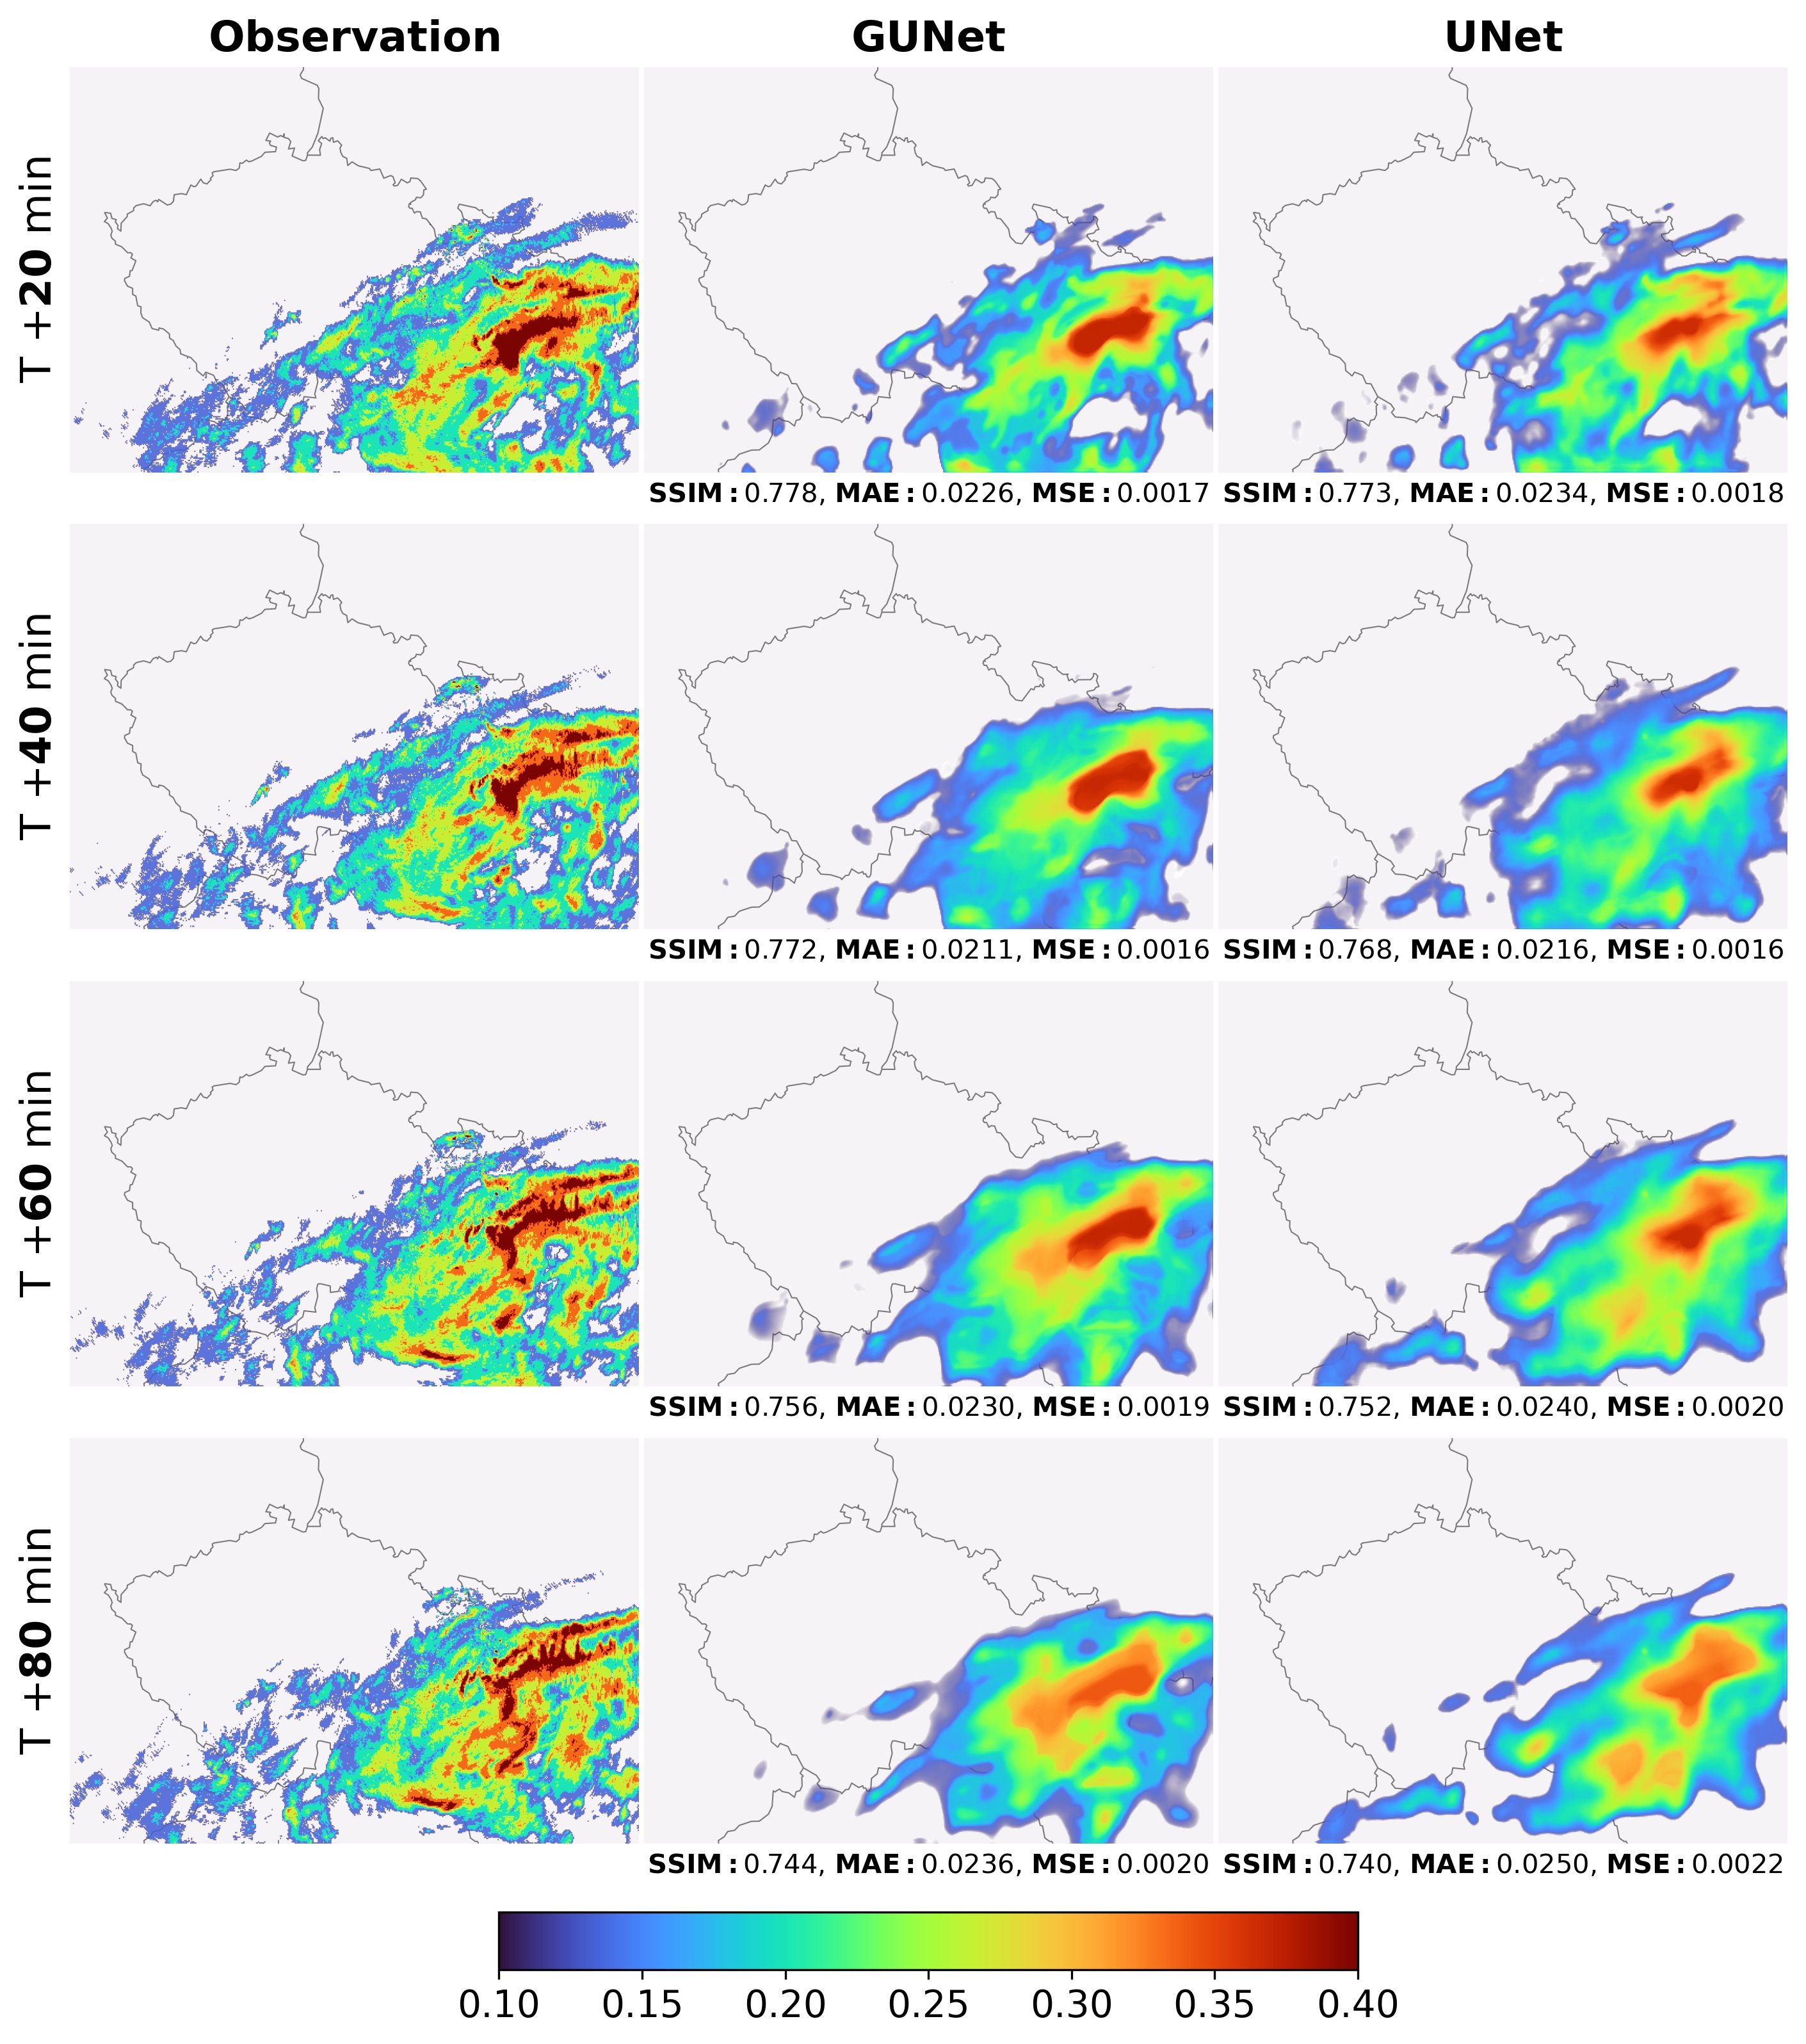
\includegraphics[width=\textwidth]{images/comparison_02.jpeg}
%     \caption[Model comparison on radar images with denser cloud formations]{\label{fig:comparison_02}Model comparison on radar images with denser cloud formations.}
% \end{figure}
%
% \begin{figure}[ht]
%     \centering
%     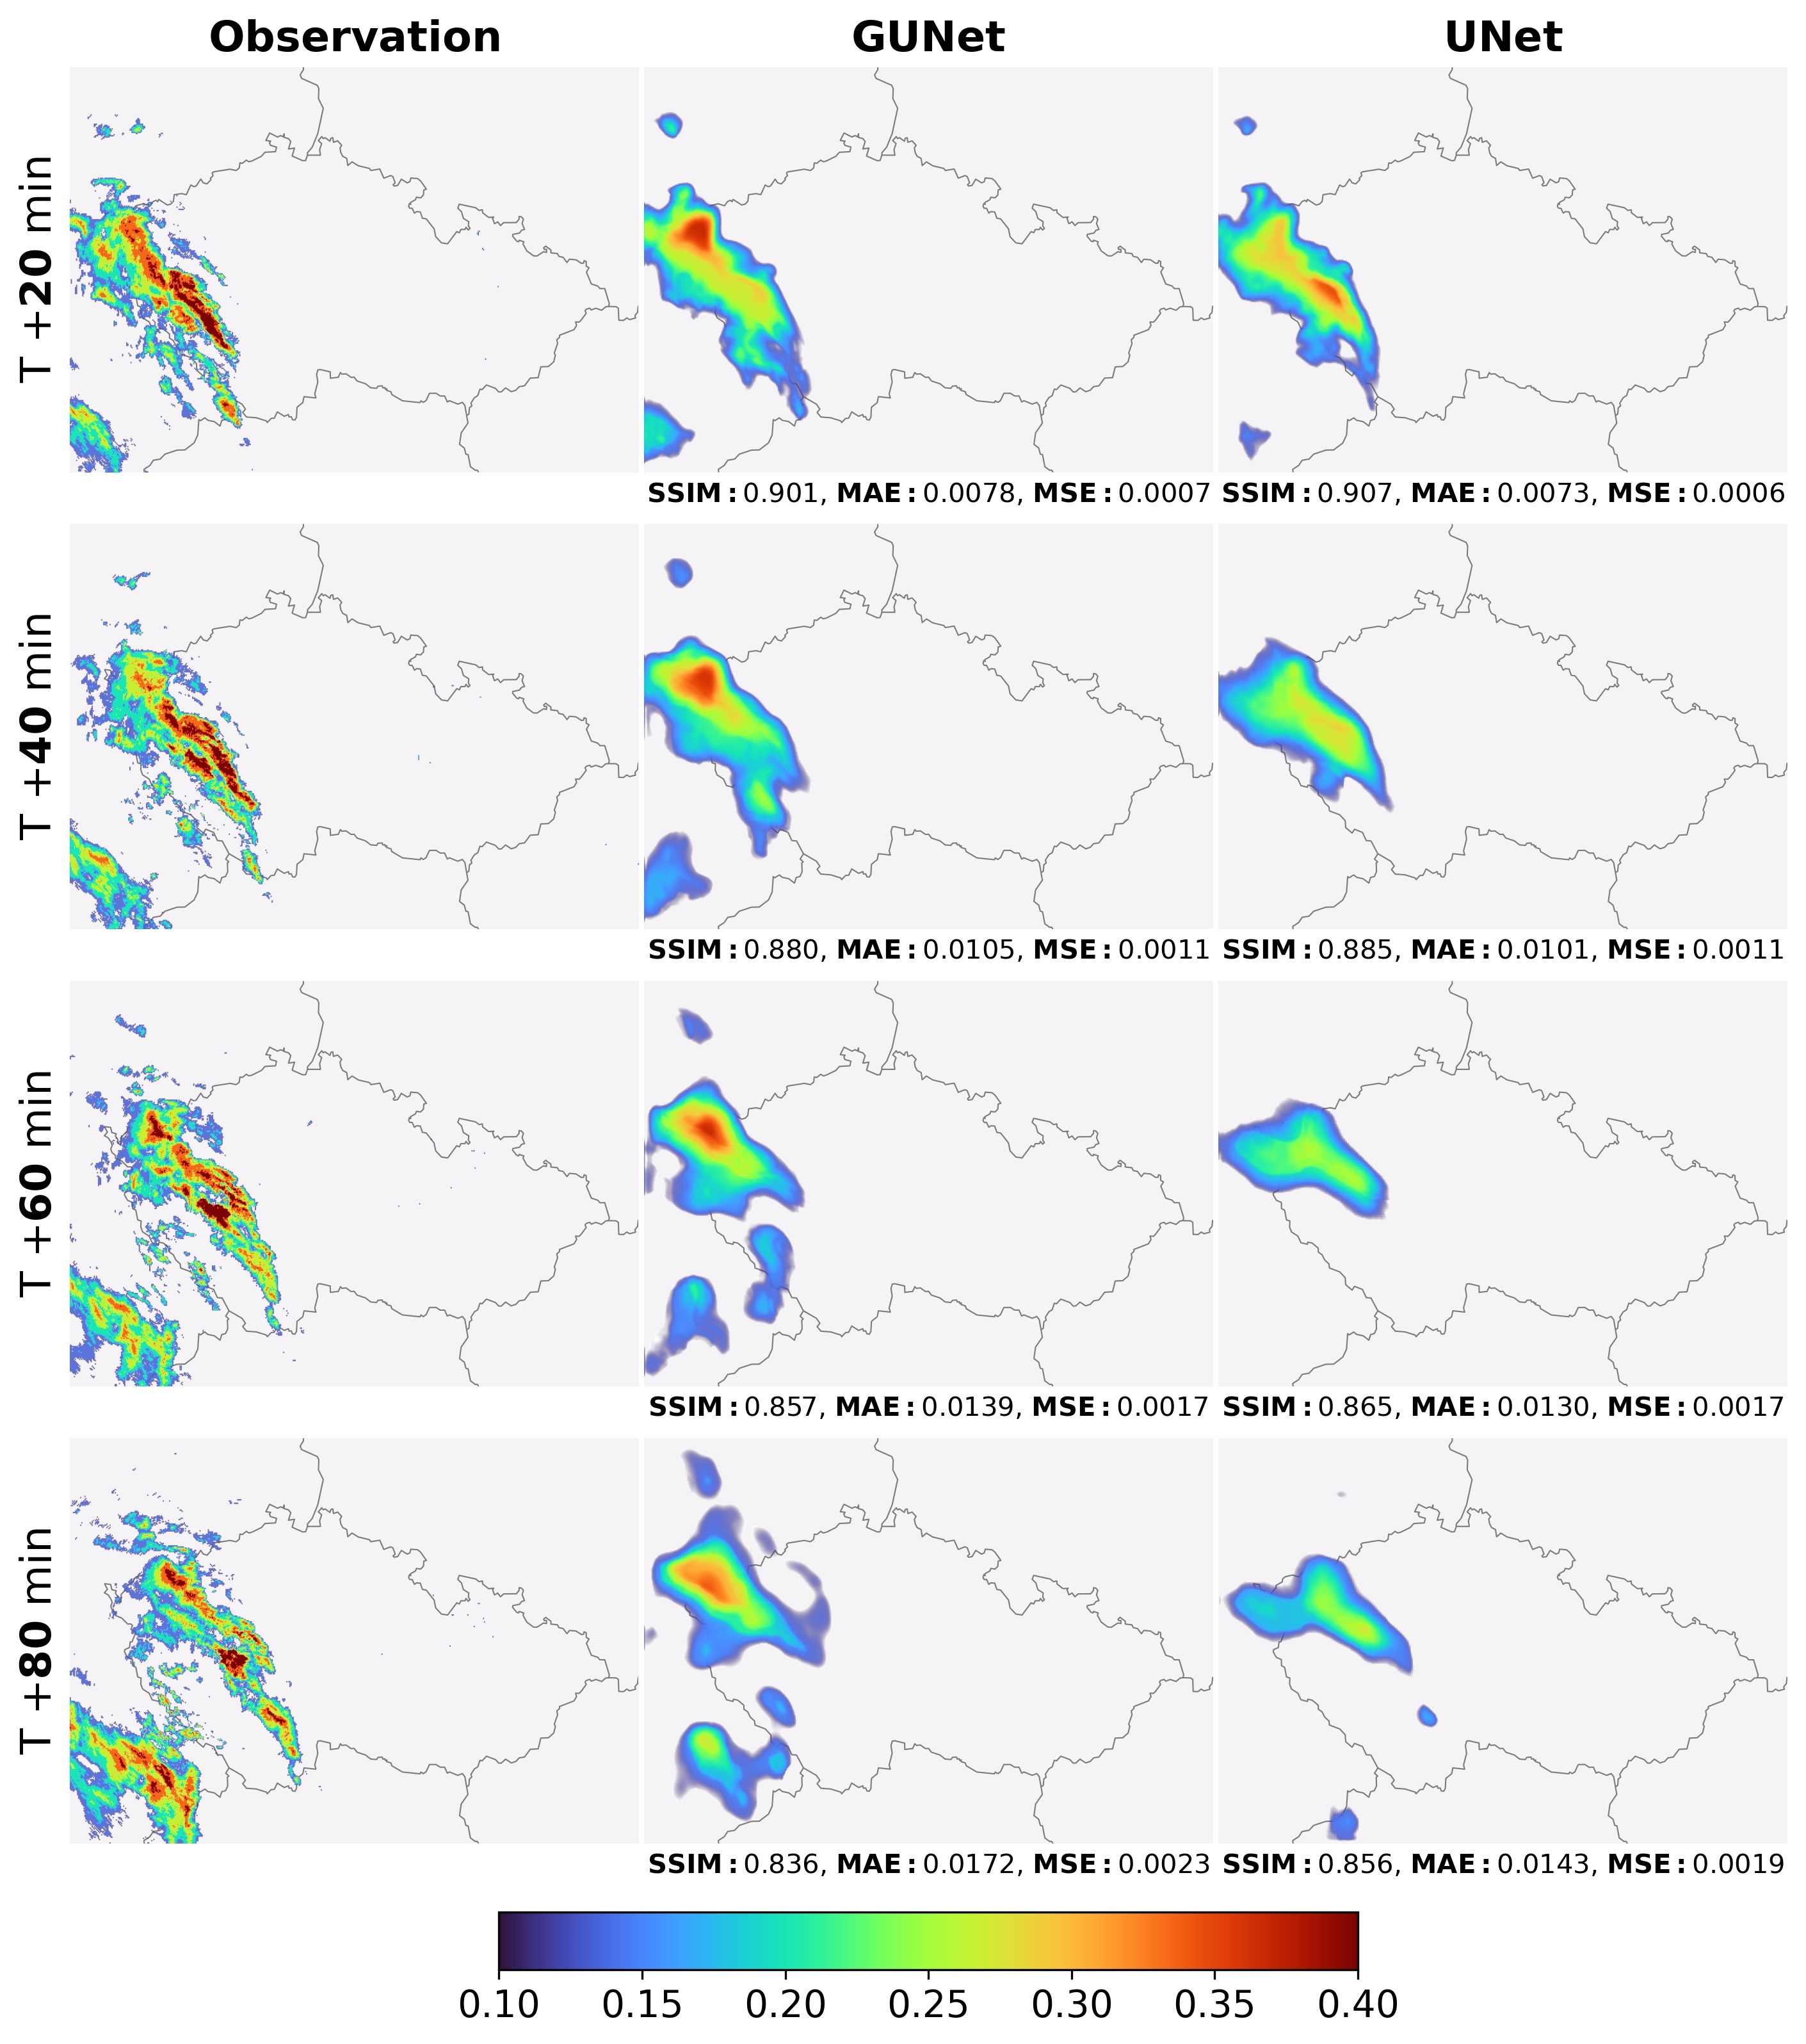
\includegraphics[width=\textwidth]{images/comparison_06.jpeg}
%     \caption[Model comparison on radar images with sparse cloud formations]{\label{fig:comparison_06}Model comparison on radar images with sparse cloud formations.}
% \end{figure}
%
% \begin{figure}[ht]
%     \centering
%     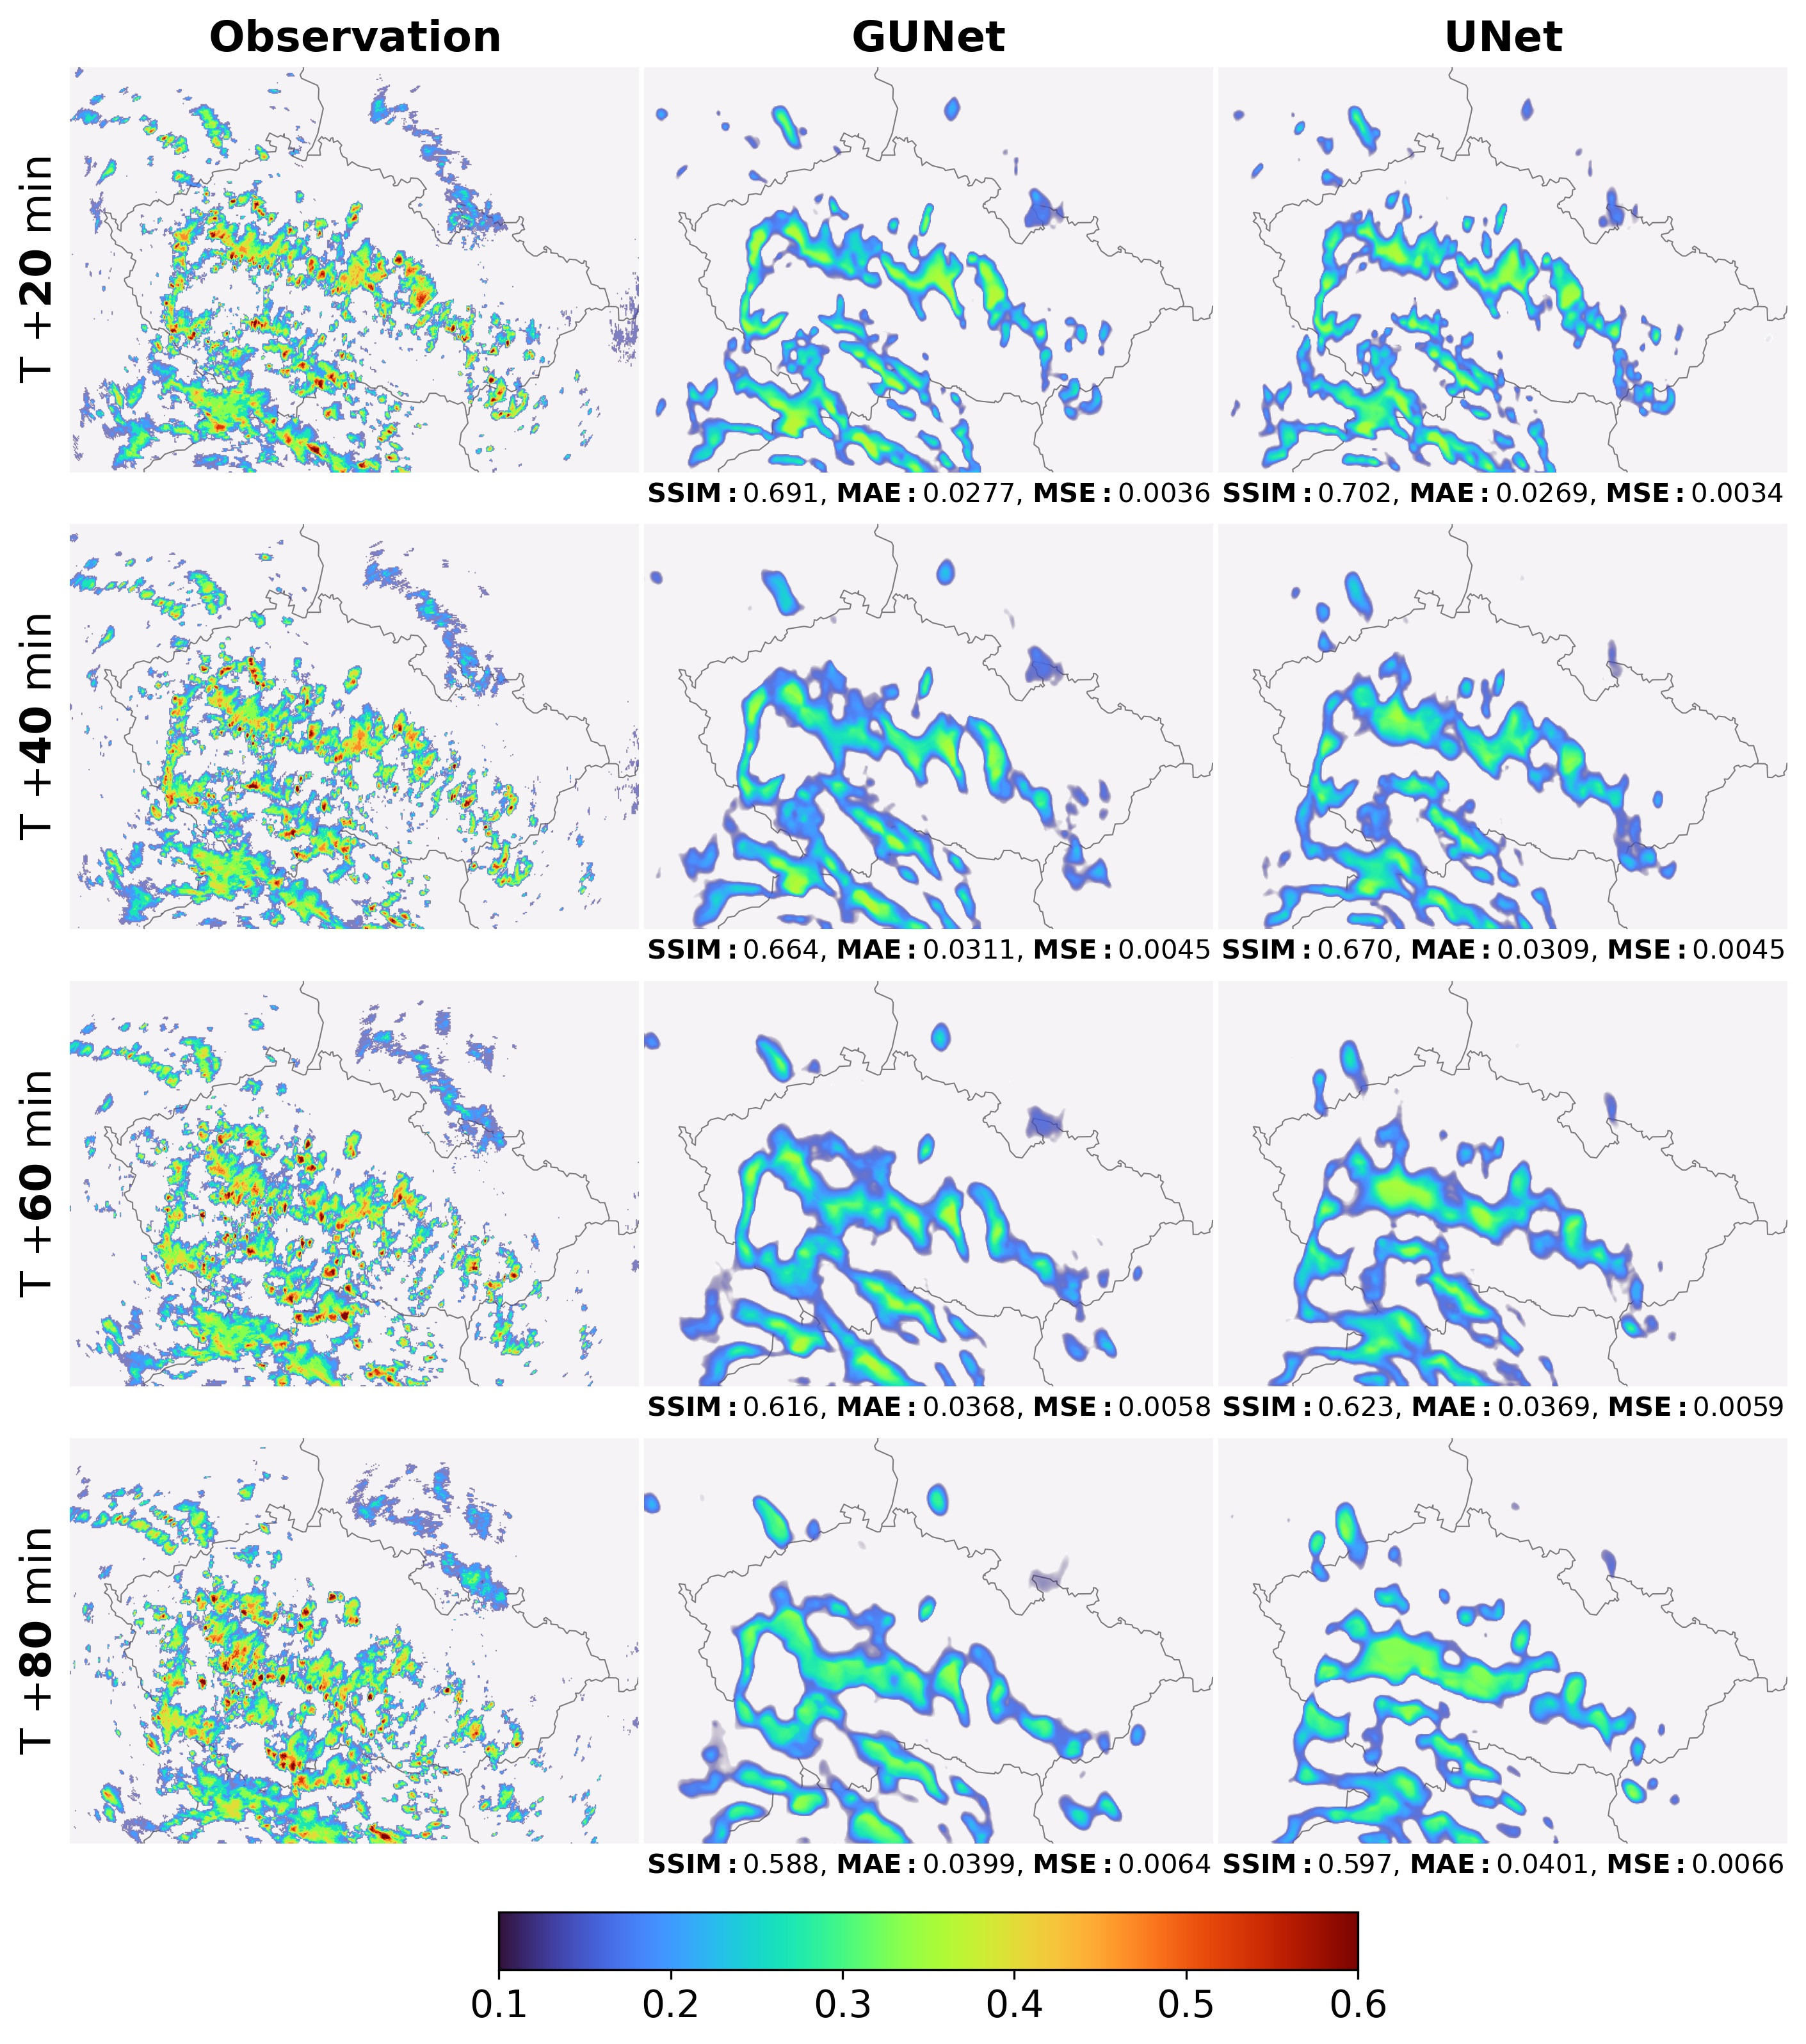
\includegraphics[width=\textwidth]{images/comparison_04.jpeg}
%     \caption[Model comparison on radar images with complex cloud formations]{\label{fig:comparison_04}Model comparison on radar images with complex cloud formations.}
% \end{figure}
%
% \begin{figure}[ht]
%     \centering
%     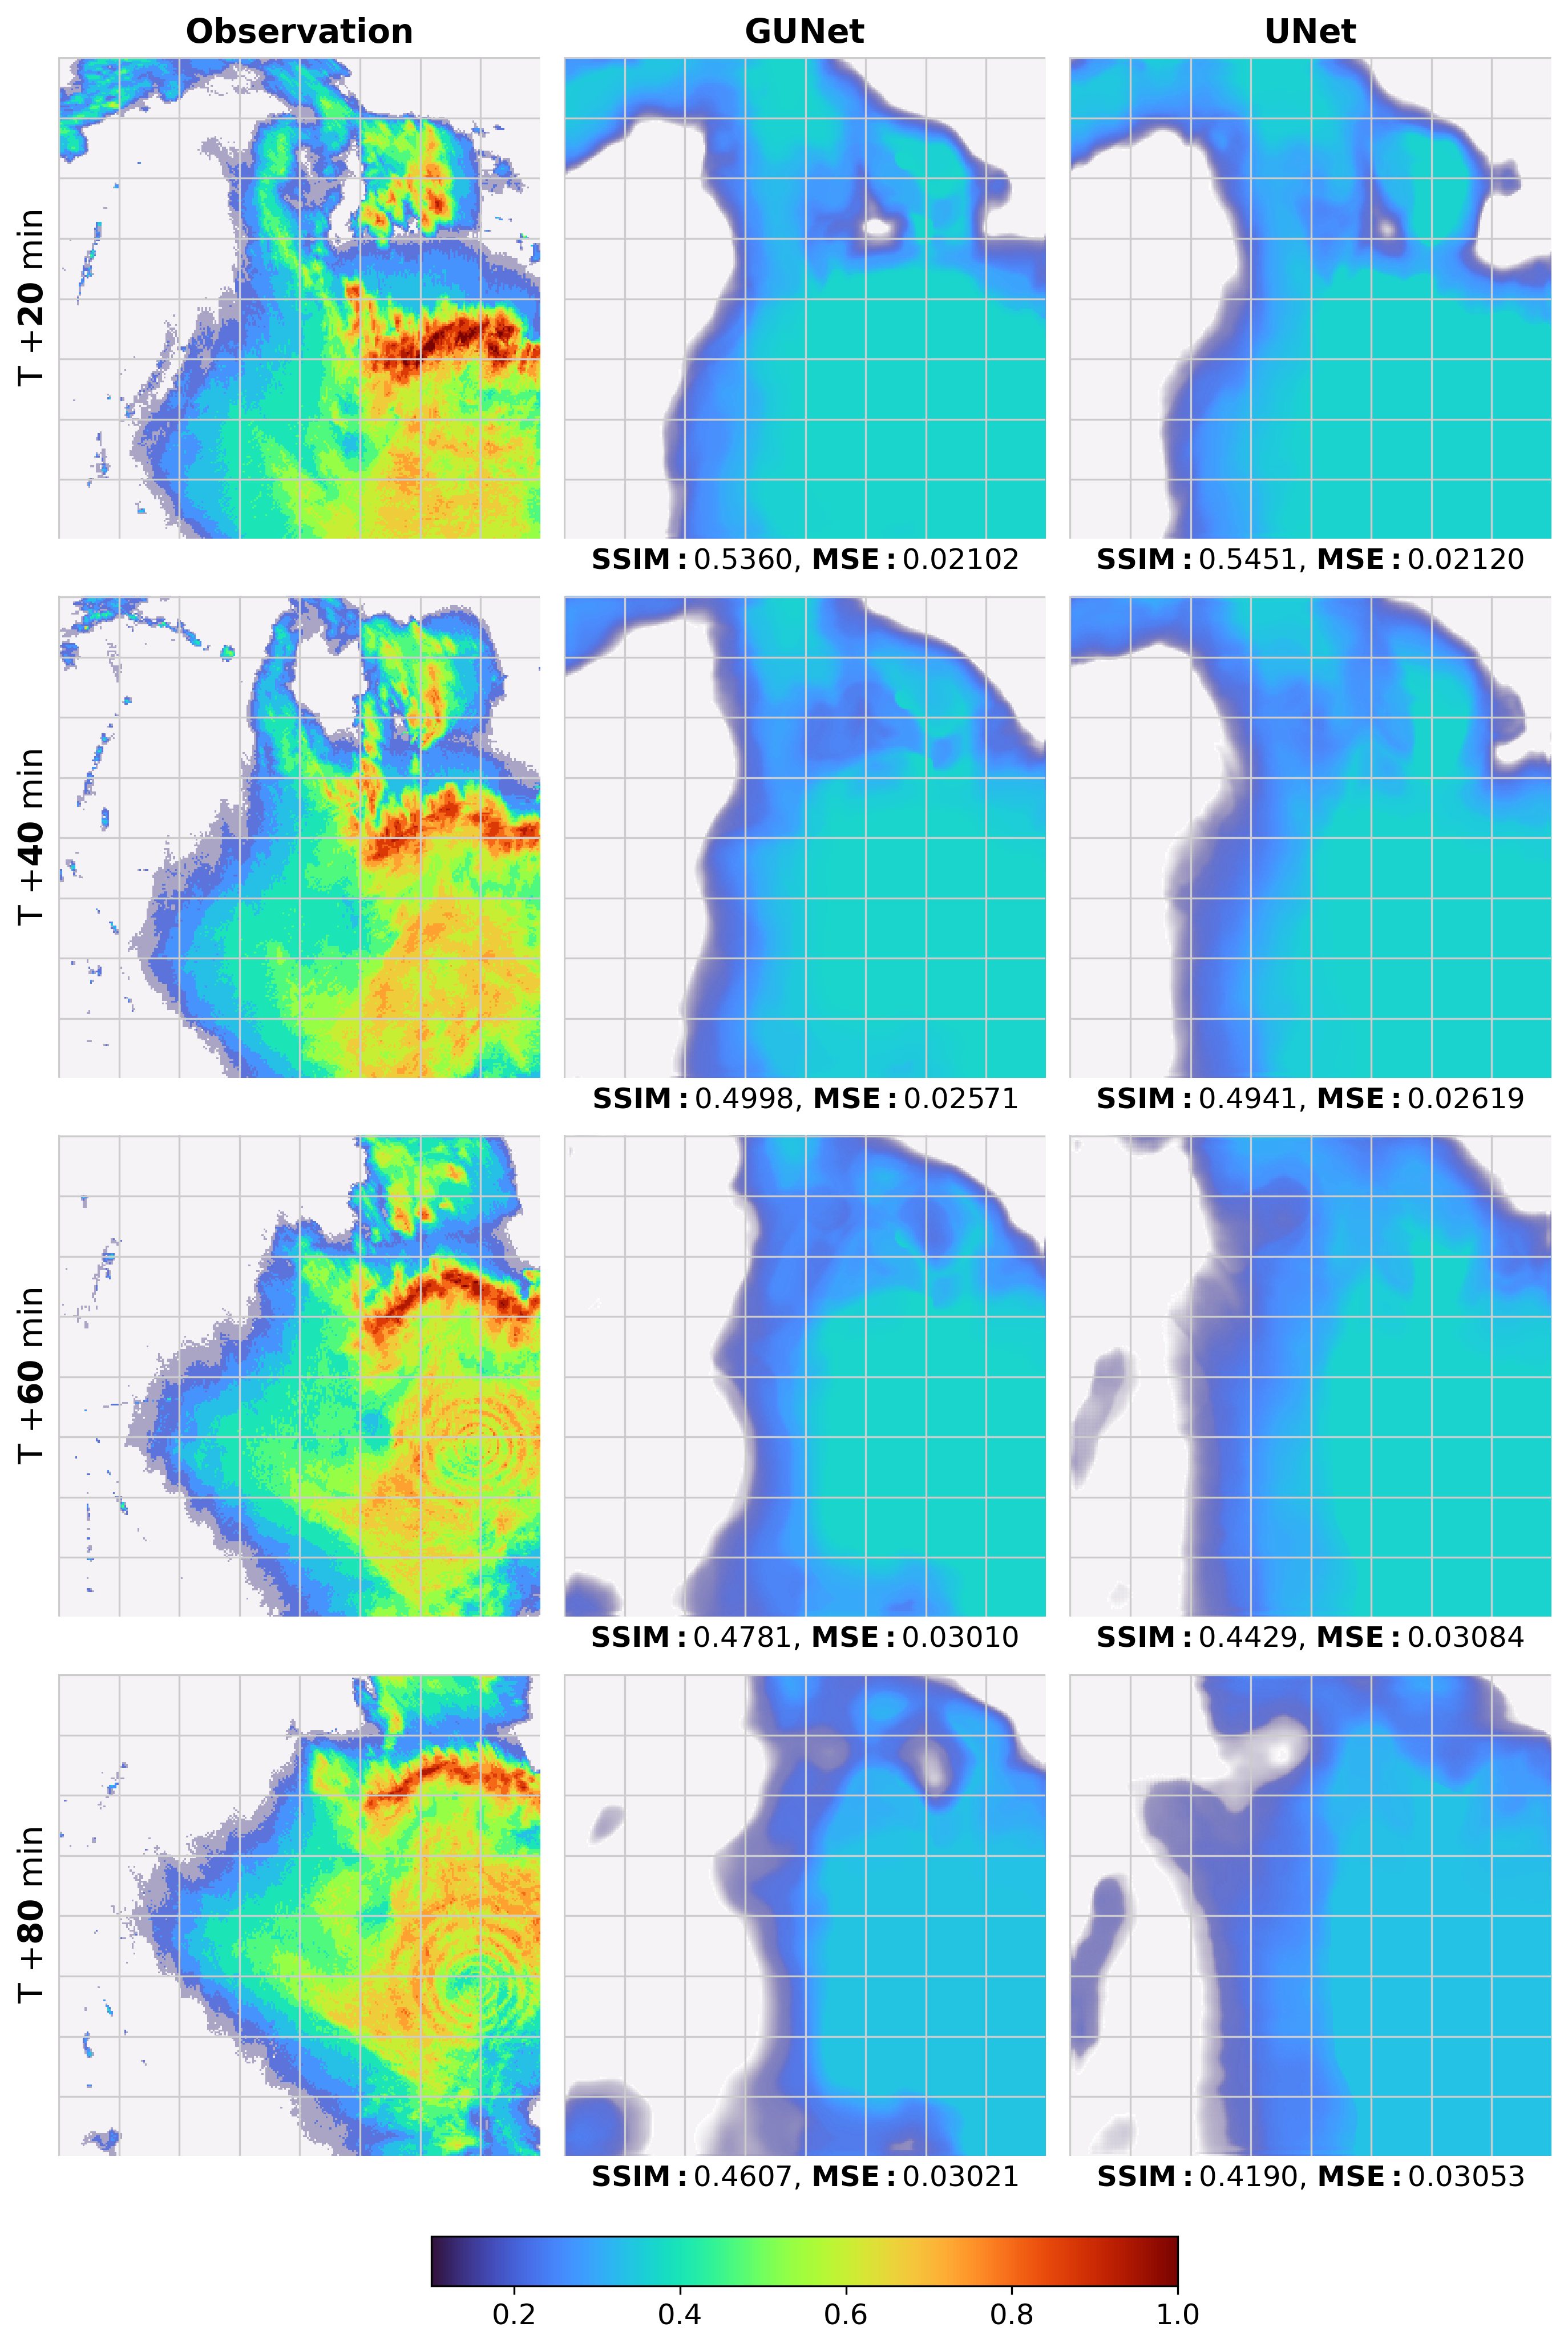
\includegraphics[width=\textwidth]{images/comparison_square_01.jpeg}
%     \caption[Model comparison on radar images with very high intensities]{\label{fig:comparison_01}Model comparison on radar images with very high echo intensities, which are not captured by either one of the models.}
% \end{figure}

\begin{figure}[ht]
    \centering
    \begin{subcaptionblock}[t]{\textwidth}
        \centering
        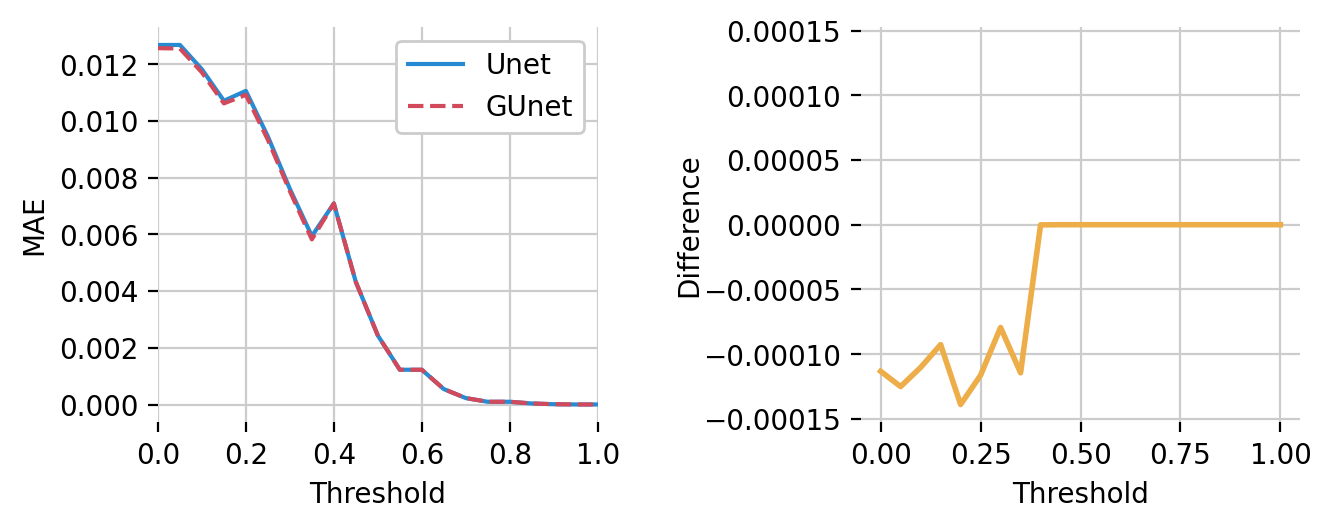
\includegraphics[width=\textwidth]{images/threshold_mae.png}
        \caption[Higher intensity storm prediction metrics]{\label{fig:threshold_mae}Average \gls{MAE} on the test dataset, computed from outputs and targets, which had some values, that were below some threshold, set to 0. Chart on the right shows the difference $\texttt{mae\_gunet} - \texttt{mae\_unet}$. Negative values mean that GUNet had better \gls{MAE}, and positive values that UNet had better \gls{MAE}.}
    \end{subcaptionblock}
    \begin{subcaptionblock}[t]{\textwidth}
        \centering
        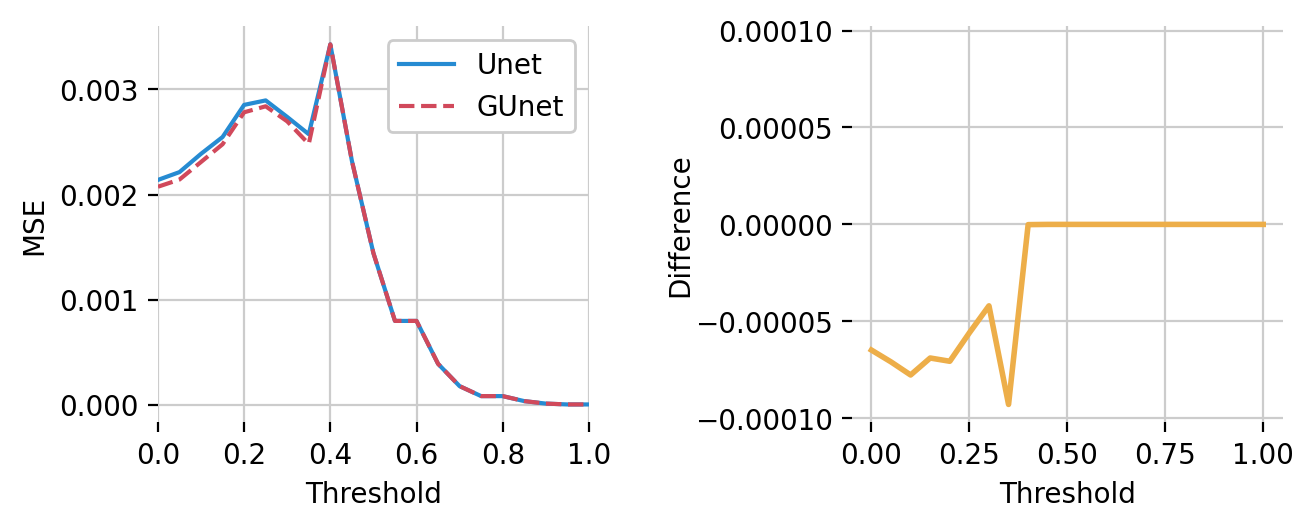
\includegraphics[width=\textwidth]{images/threshold_mse.png}
        \caption[Higher intensity storm prediction metrics]{\label{fig:threshold_mse}Average \gls{MSE} on the test dataset, computed from outputs and targets, which had some values, that were below some threshold, set to 0. Chart on the right shows the difference $\texttt{mse\_gunet} - \texttt{mse\_unet}$. Negative values signify better GUNet \gls{MSE}.}
    \end{subcaptionblock}
\end{figure}


\begin{figure}[ht]
    \centering
    \begin{subcaptionblock}[t]{\textwidth}
        \centering
        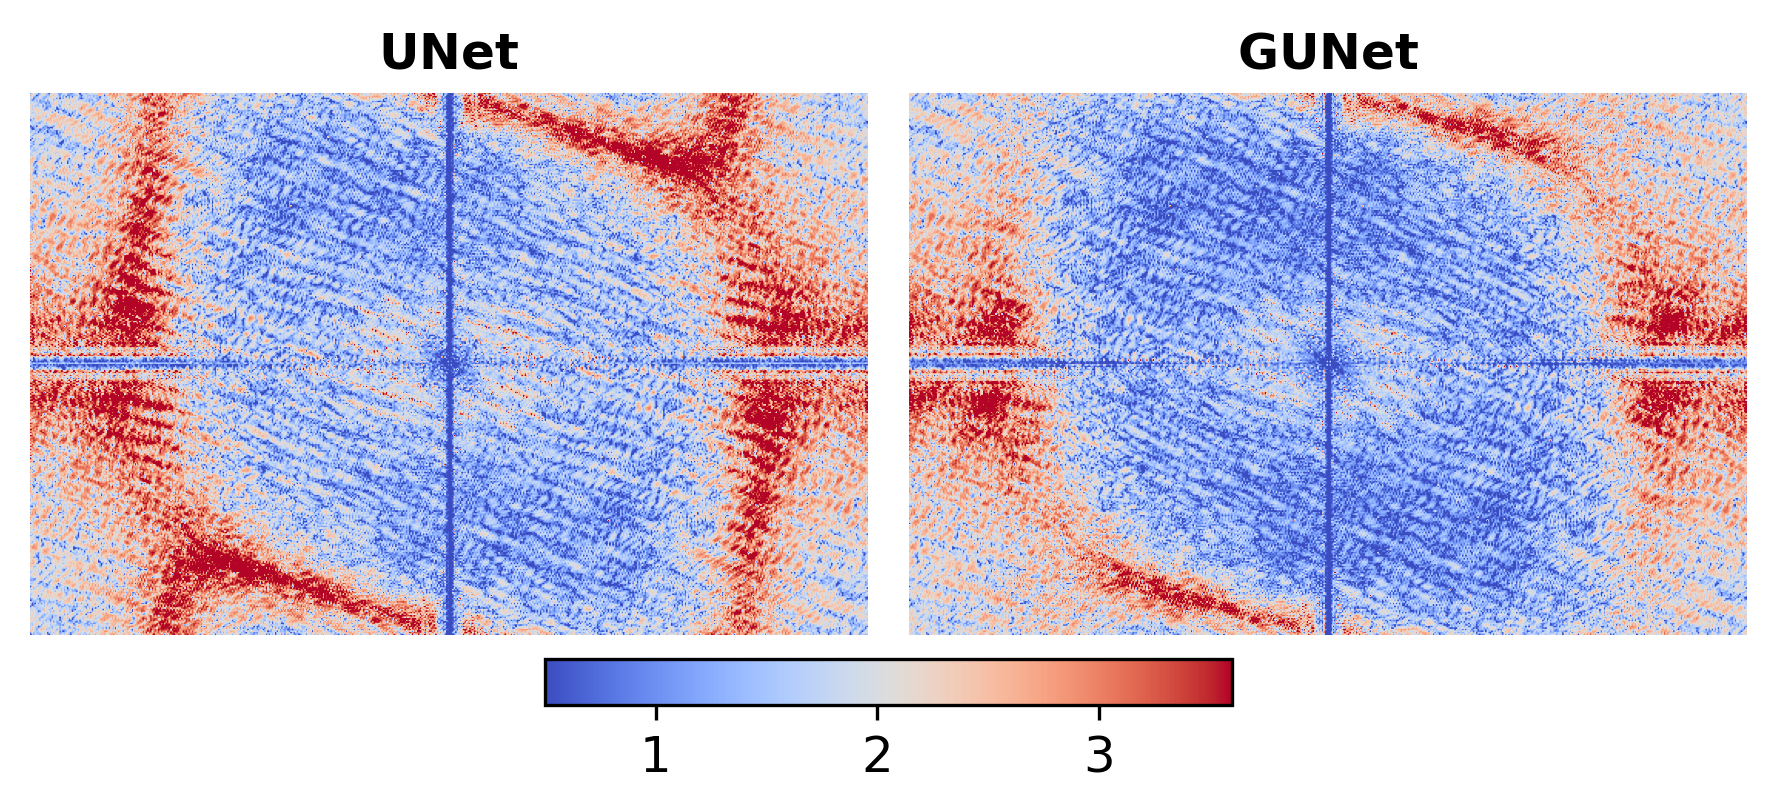
\includegraphics[width=\textwidth]{images/fourier_diff_2.png}
        \caption[Delta of the target and output spectra without smoothing]{\label{fig:fourier_diff_2}Absolute difference between the amplitudes of the average target spectrum $\bar{M}_{\texttt{tgt}}$ and the average output spectra of the models $\bar{M}_{\texttt{UNet}}$ and $\bar{M}_{\texttt{GUNet}}$, on a logarithmic scale. Higher value of a pixel means, that the amplitude at the frequency corresponging to that pixel, differed more from the desired amplitude of average target spectra $\bar{M}_{\texttt{tgt}}$. }
    \end{subcaptionblock}
    \begin{subcaptionblock}[t]{\textwidth}
        \centering
        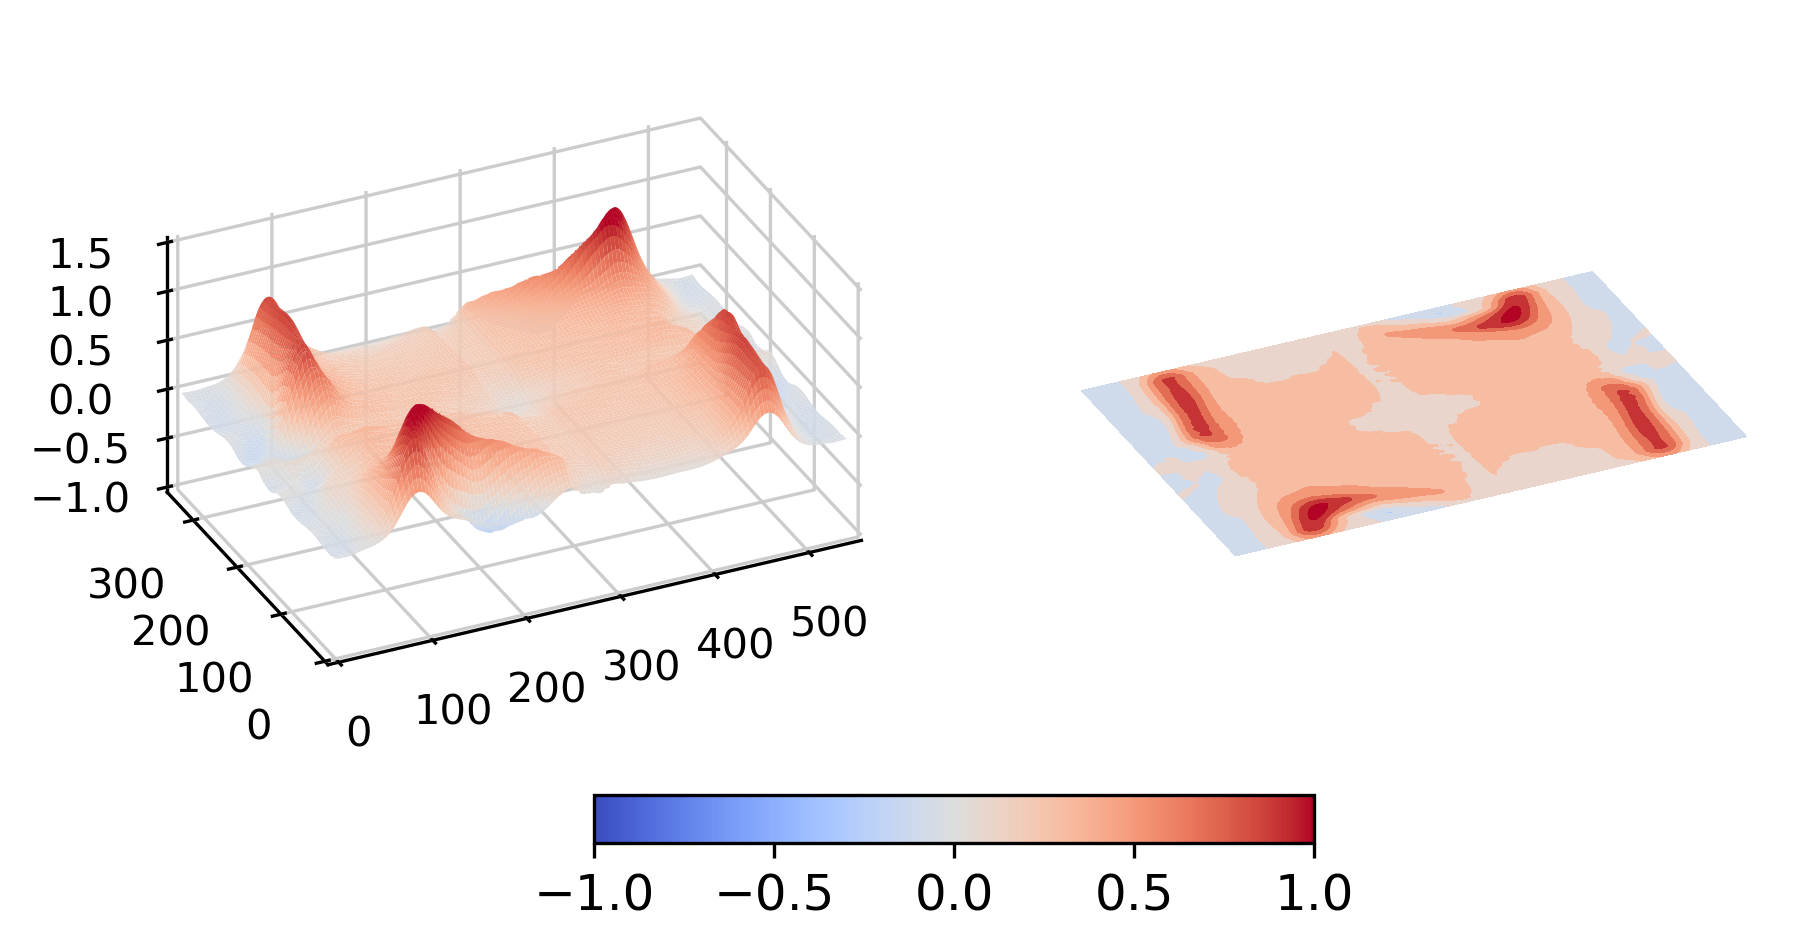
\includegraphics[width=\textwidth]{images/fourier_diff_3.png}
        \caption[Difference in the output spectra of both models]{\label{fig:fourier_diff_3}Amplitudes of the average UNet output spectrum $\bar{M}_{\texttt{UNet}}$ subtracted from the amplitudes of the average GUNet outputs $\bar{M}_{\texttt{GUNet}}$ on a logarithmic scale. Values were passed through moving average with kernel size 32×32. Higher value of a pixel means, that GUNet outputs had higher average amplitude than the UNet outputs, at the frequency corresponging to the given pixel.}
    \end{subcaptionblock}
\end{figure}


\begin{figure}[ht]
    \centering
    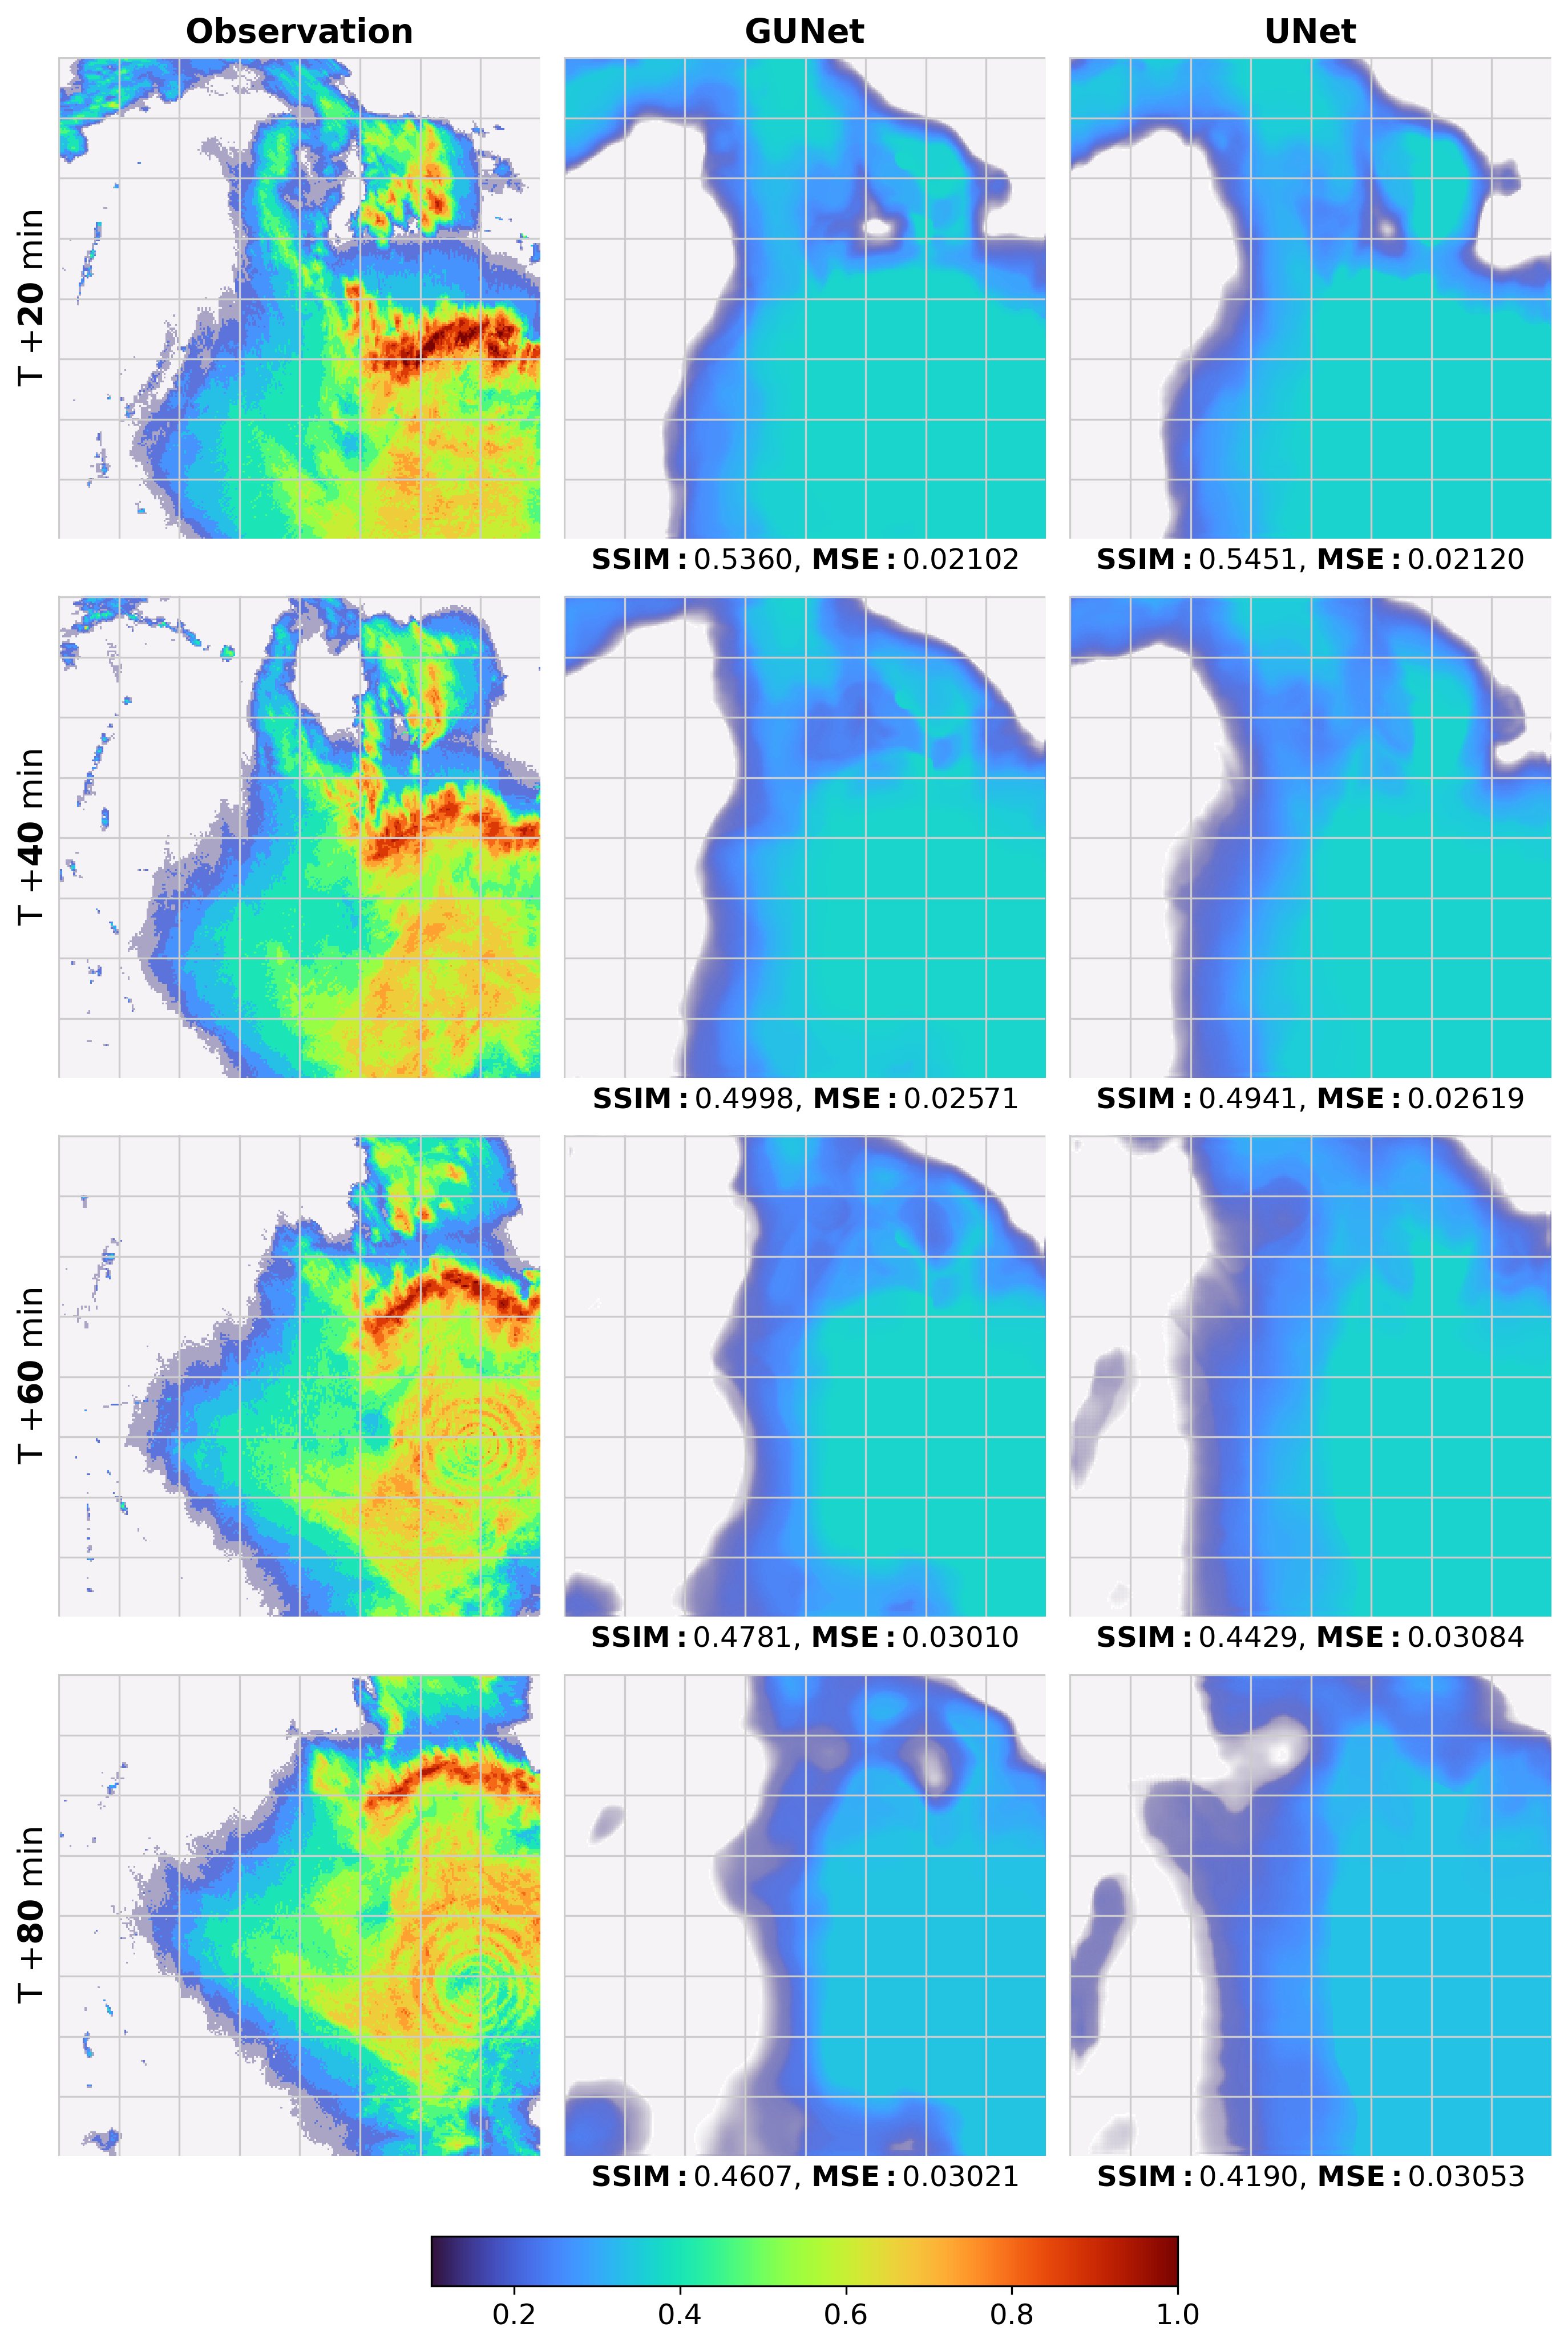
\includegraphics[width=\textwidth]{images/comparison_square_01.png}
    \caption[Comparison of weather predictions of both models (2)]{\label{fig:comparison_01}Model comparison on radar images with very high echo intensities, which are not captured by either one of the models.}
\end{figure}

\begin{figure}[ht]
    \centering
    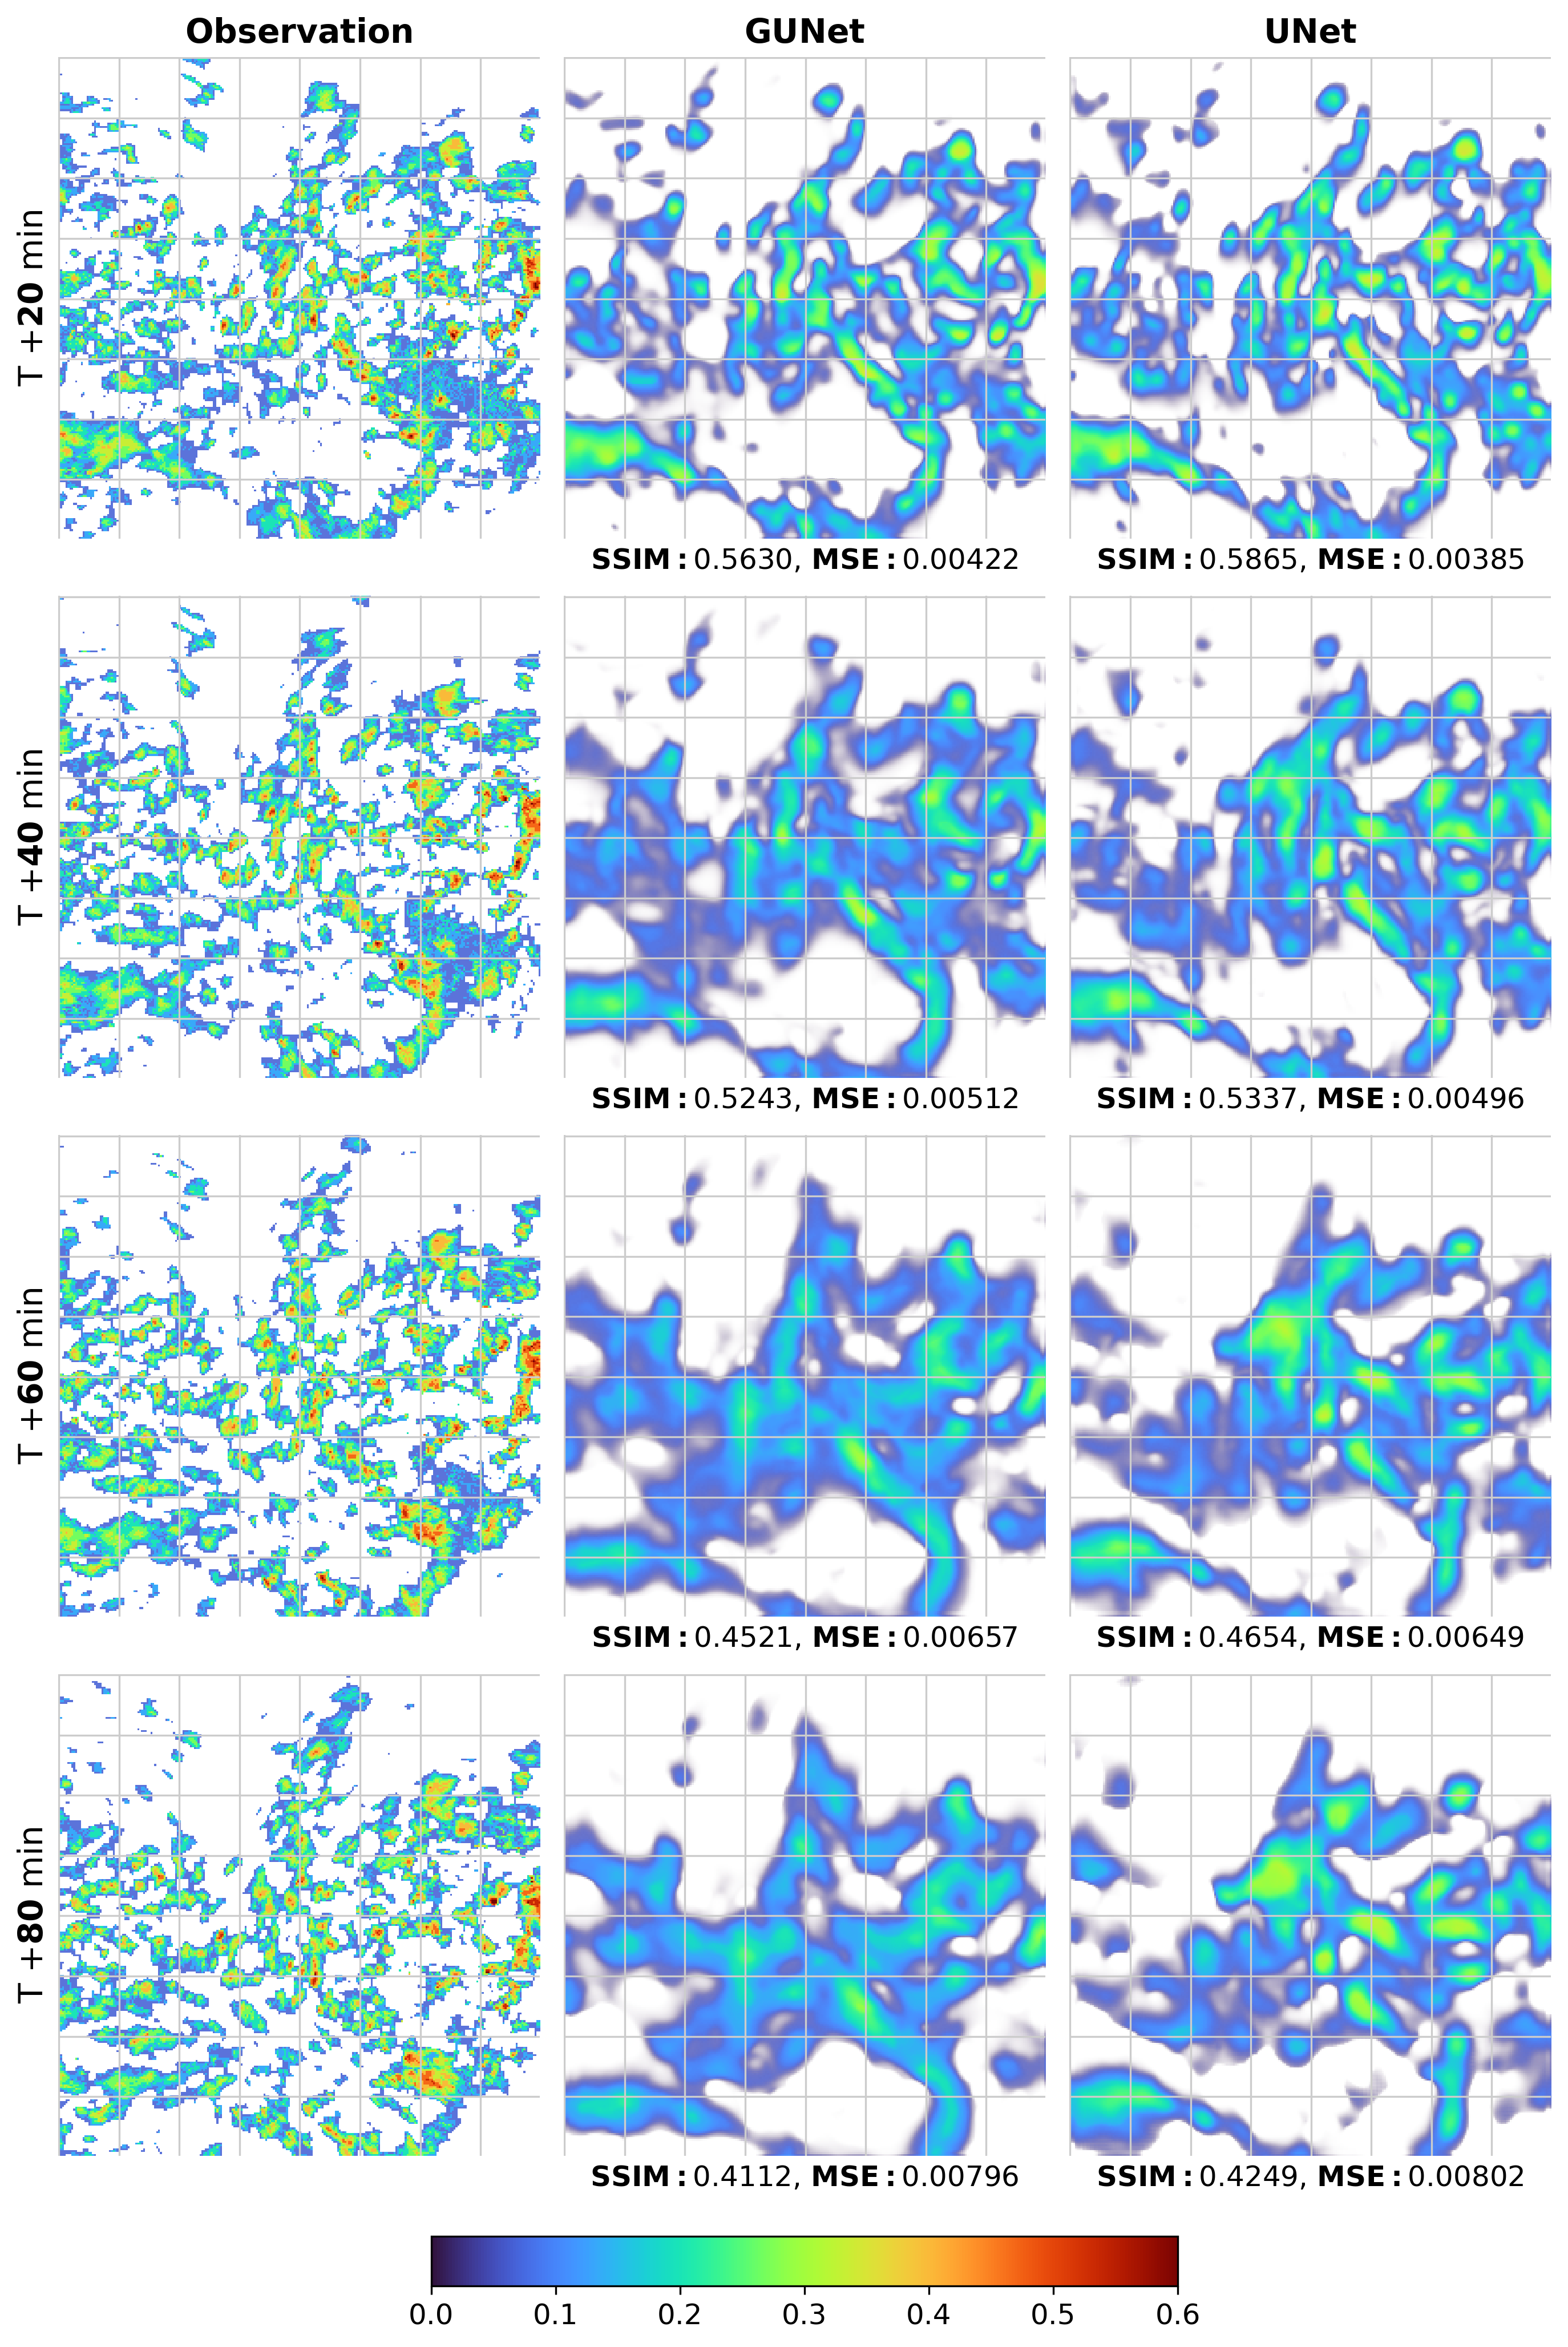
\includegraphics[width=\textwidth]{images/comparison_square_09.png}
    \caption[Comparison of weather predictions of both models (3)]{\label{fig:comparison_09}Model comparison on radar images with complex cloud formations.}
\end{figure}

\begin{figure}[ht]
    \centering
    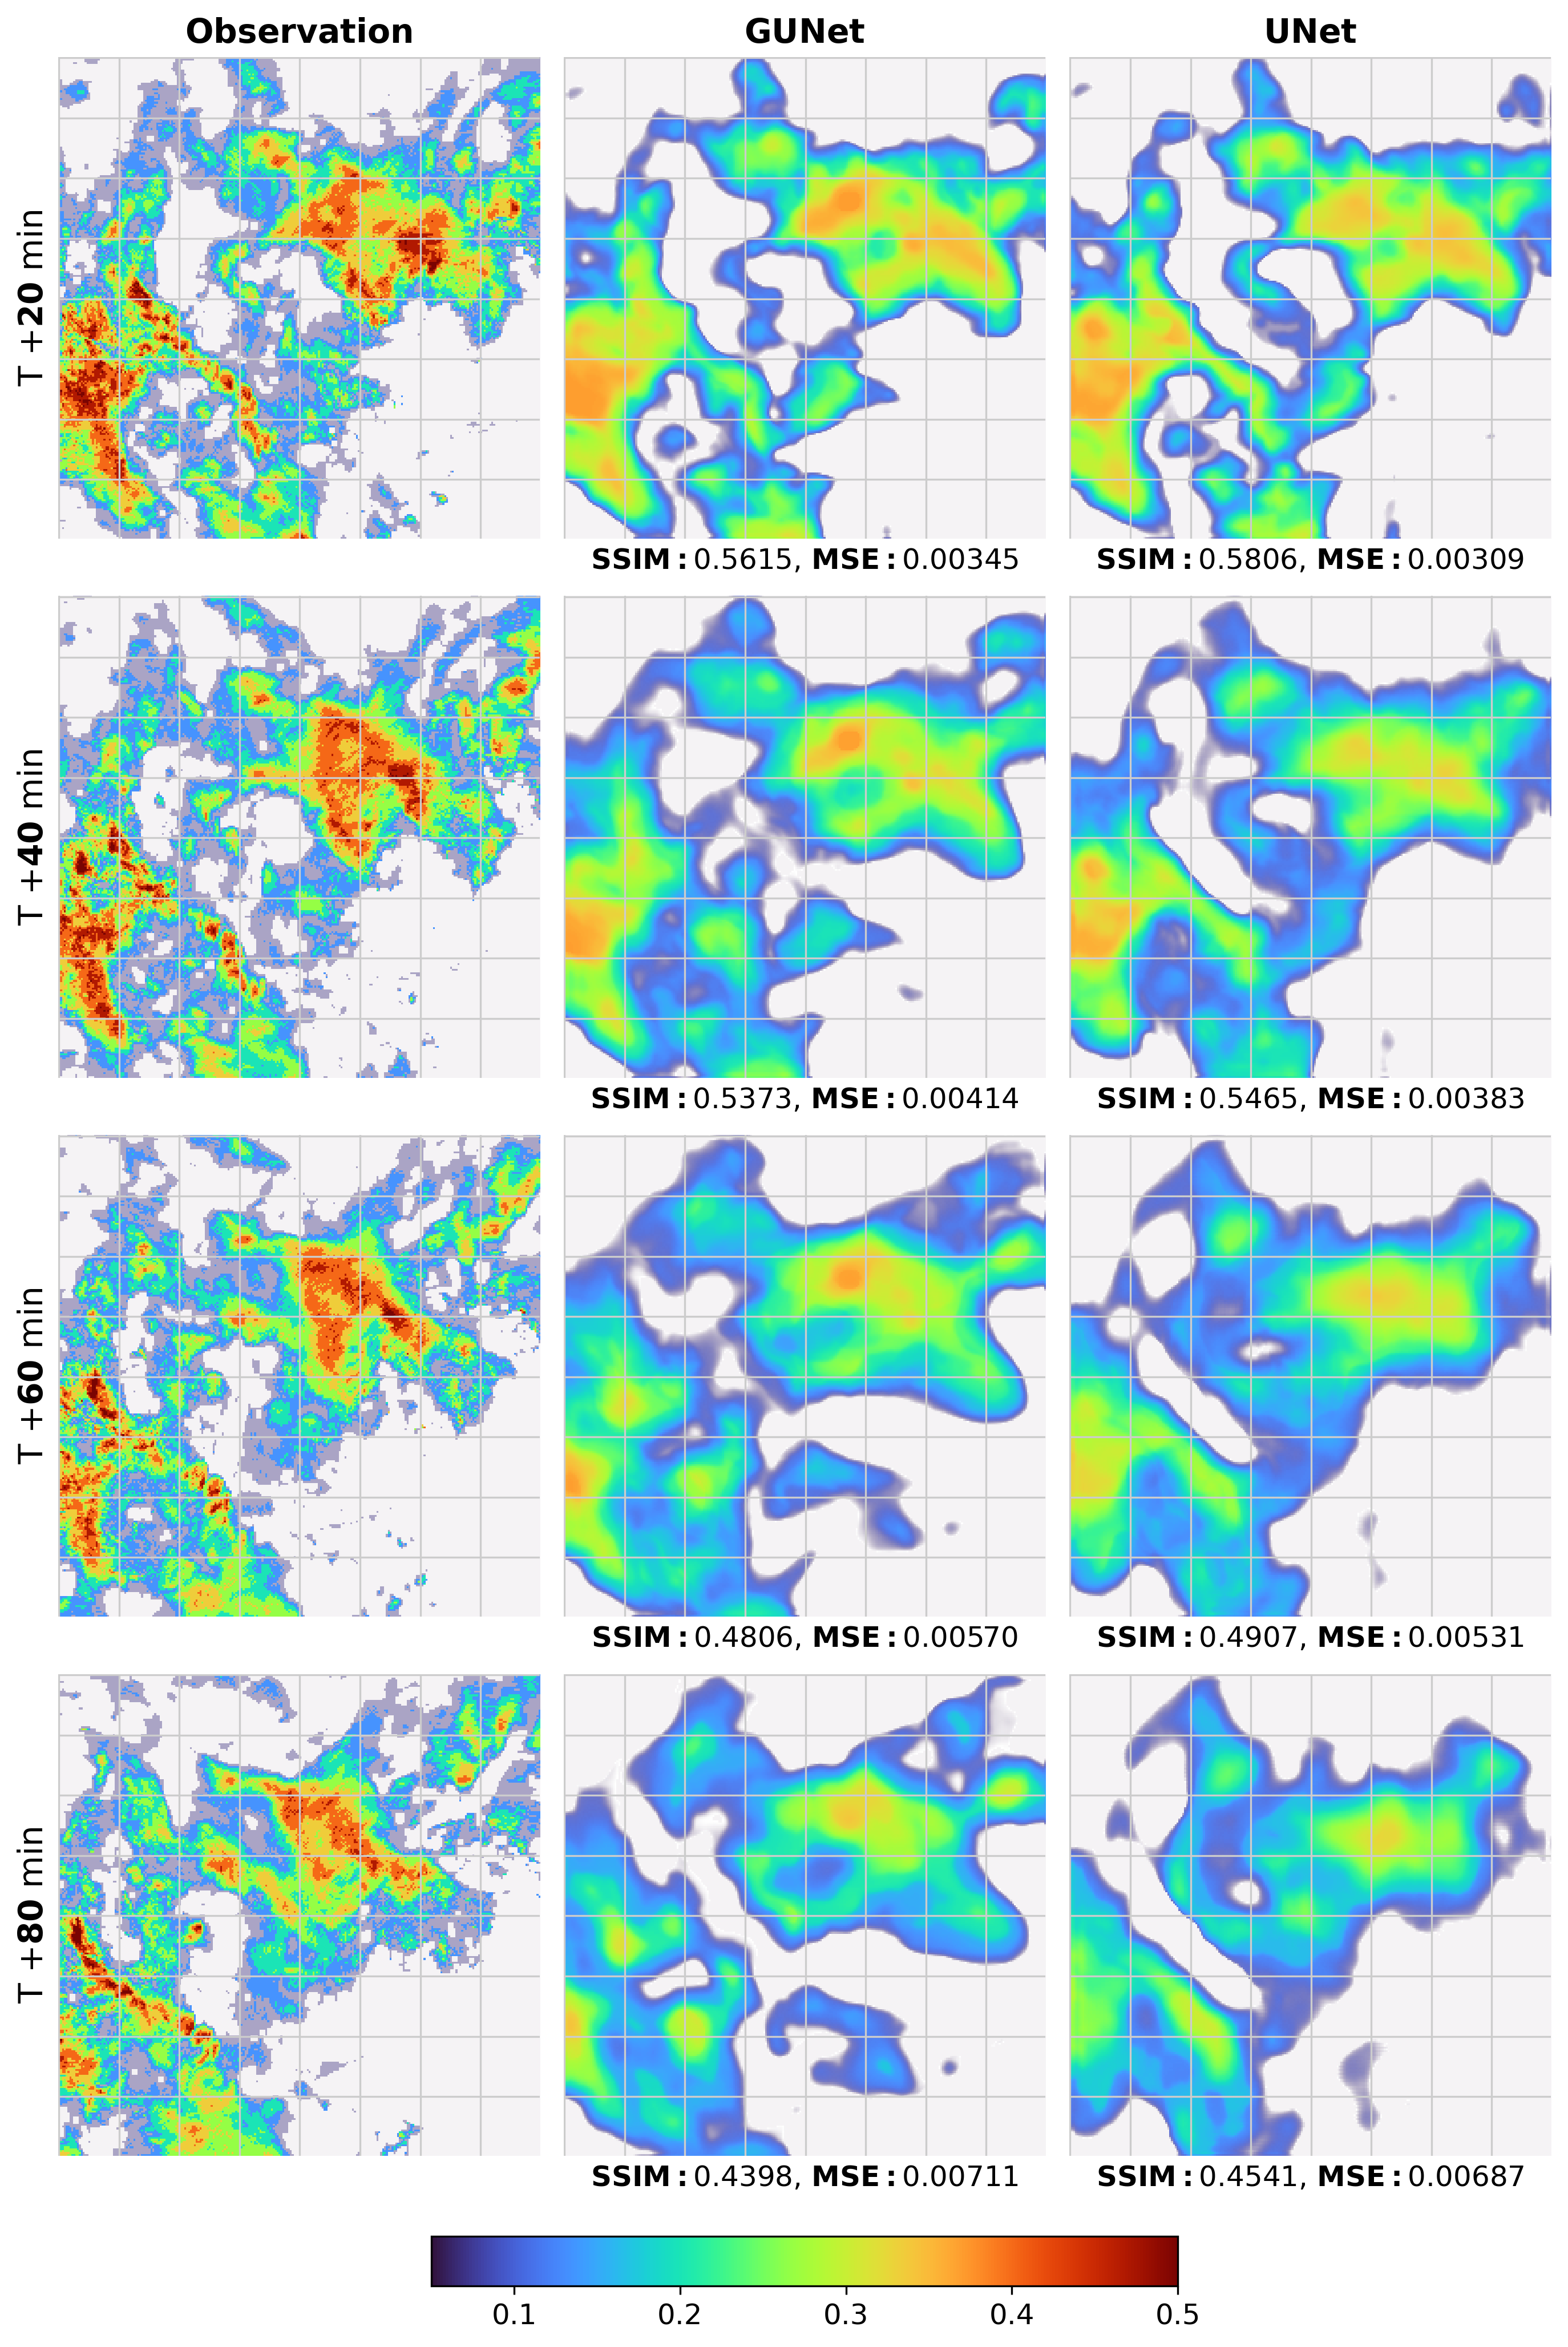
\includegraphics[width=\textwidth]{images/comparison_square_07.png}
    \caption[Comparison of weather predictions of both models.(4)]{\label{fig:comparison_07}}
\end{figure}

\begin{figure}[ht]
    \centering
    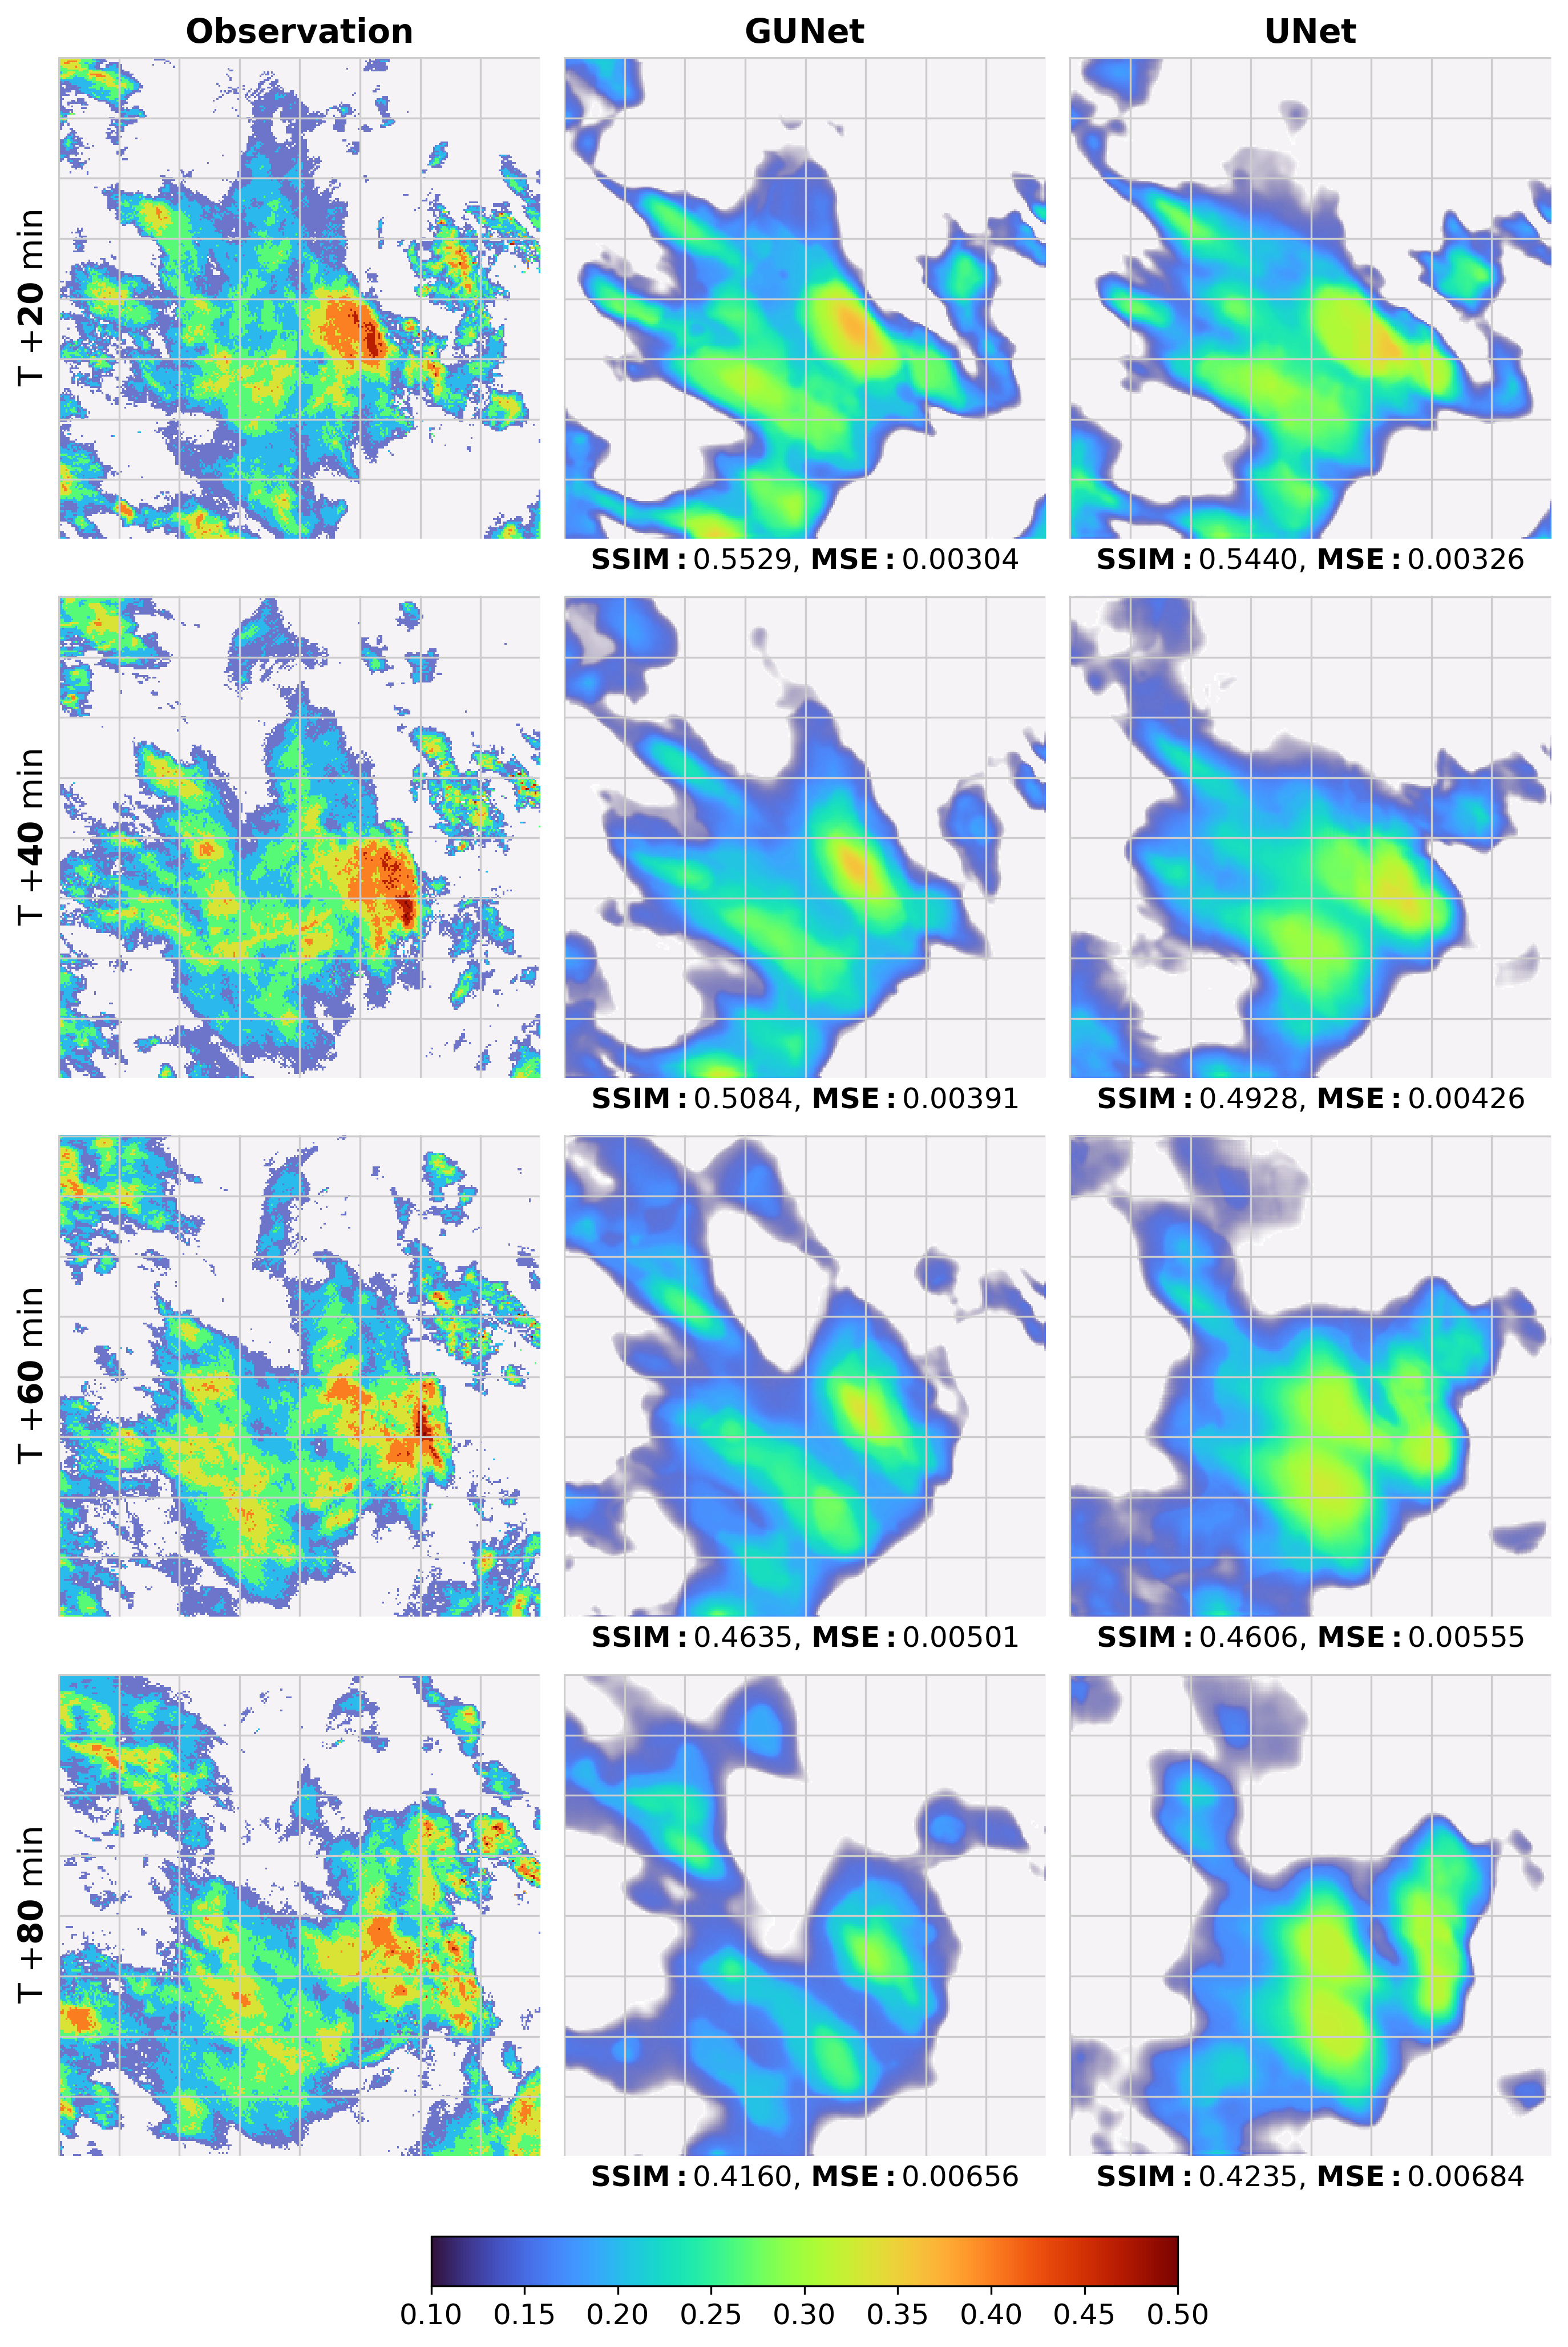
\includegraphics[width=\textwidth]{images/comparison_square_04.png}
    \caption[Comparison of weather predictions of both models (5)]{\label{fig:comparison_04}}
\end{figure}

\chapter{Acronyms}
\renewcommand{\glossarysection}[2][]{}
\printglossaries

\chapter{Contents of the Archive}

%change appropriately

\begin{figure}[h]
    \dirtree{%
    .1 README.md\DTcomment{information about the contents of the archive}.
    .1 src\DTcomment{directory containing the implementation}.
    .2 dataset.py\DTcomment{script for generating the datasets}.
    .2 tuning.py\DTcomment{script for hyperparameter tuning}.
    .2 train.py\DTcomment{model trainining script}.
    .2 gunet.py\DTcomment{implementation of GUNet in PyTorch}.
    .2 unet.py\DTcomment{implementation of UNet in PyTorch}.
    .2 gunet\_weights\_best.pt\DTcomment{weights of the best GUNet}.
    .2 unet\_weights\_best.pt\DTcomment{weights of the best UNet}.
    .2 visualization.ipynb\DTcomment{notebook used for creating the visualizations}.
    .1 thesis\DTcomment{directory containing the text}.
    .2 chapters\DTcomment{directory containing text of the chapters}.
    .2 images\DTcomment{directory containing images used in the thesis}.
    .2 thesis.tex\DTcomment{main \LaTeX{} source file}.
    .2 bibliography.bib\DTcomment{bibliography}.
    .2 thesis.pdf\DTcomment{this pdf}.
    }
\end{figure}
